\documentclass[
	a4paper,
	pagesize,
	pdftex,
	12pt,
	twoside, % + BCOR darunter: für doppelseitigen Druck aktivieren, sonst beide deaktivieren
	BCOR=5mm, % Dicke der Bindung berücksichtigen (Copyshop fragen, wie viel das ist)
	ngerman,
	fleqn,
	final,
	]{scrartcl}
\usepackage{ucs}
\usepackage[utf8x]{inputenc} % Eingabekodierung: UTF-8
\usepackage{fixltx2e} % Schickere Ausgabe
\usepackage[T1]{fontenc} % ordentliche Trennung
\usepackage[ngerman]{babel}
\usepackage{lmodern} % ordentliche Schriften
\usepackage[unicode=true]{hyperref}
\usepackage{setspace,graphicx,tikz,tabularx} % für Elemente der Titelseite
\usepackage[draft=false,babel,tracking=true,kerning=true,spacing=true]{microtype} % optischer Randausgleich etc.

\usepackage{amsmath}
\usepackage{ amssymb }
\usepackage{todonotes}
\usepackage{ dsfont }
\usepackage{subcaption}
\usepackage{wrapfig}
\usepackage{blindtext}
\usepackage{scrextend}
\addtokomafont{labelinglabel}{\sffamily}


\usepackage[figurename=Figure]{caption}
\begin{document}

% Beispielhafte Nutzung der Vorlage für die Titelseite (bitte anpassen):
% LaTeX-Vorlage für die Titelseite und Selbständigkeitserklärung einer Abschlussarbeit
% basierend auf der vorigen Institutsvorlage des Instituts für Informatik
% sowie der Vorlage für Promotionsarbeiten.
%
% erweitert: 2014-06-12 Dennis Schneider <dschneid@informatik.hu-berlin.de>

% gepunktete Linie unter Objekt:
\newcommand{\TitelPunkte}[1]{%
  \tikz[baseline=(todotted.base)]{
    \node[inner sep=1pt,outer sep=0pt] (todotted) {#1};
    \draw[dotted] (todotted.south west) -- (todotted.south east);
  }%
}%

% gepunktete Linie mit gegebener Länge:
\newcommand{\TitelPunktLinie}[1]{\TitelPunkte{\makebox[#1][l]{}}}

\makeatletter

\newcommand*{\@titelTitel}{Titel der Arbeit}
\newcommand{\titel}[1]{\renewcommand*{\@titelTitel}{#1}} % Titel der Arbeit
\newcommand*{\@titelArbeit}{Arbeitstyp}
\newcommand{\typ}[1]{\renewcommand*{\@titelArbeit}{#1}} % Typ der Arbeit
\newcommand*{\@titelGrad}{akademischer Grad}
\newcommand{\grad}[1]{\renewcommand*{\@titelGrad}{#1}} % Akademischer Grad
\newcommand*{\@titelAutor}{Autor}
\newcommand{\autor}[1]{\renewcommand*{\@titelAutor}{#1}} % Autor der Arbeit
\newcommand*{\@titelGeburtsdatum}{\TitelPunktLinie{2cm}}
\newcommand{\gebdatum}[1]{\renewcommand*{\@titelGeburtsdatum}{#1}} % Geburtsdatum des Autors
\newcommand*{\@titelGeburtsort}{\TitelPunktLinie{5cm}}
\newcommand{\gebort}[1]{\renewcommand*{\@titelGeburtsort}{#1}} % Geburtsort des Autors
\newcommand*{\@titelGutachterA}{\TitelPunktLinie{5cm}}
\newcommand*{\@titelGutachterB}{\TitelPunktLinie{5cm}}
\newcommand{\gutachter}[2]{\renewcommand*{\@titelGutachterA}{#1}\renewcommand*{\@titelGutachterB}{#2}} % Erst- und Zweitgutachter
\newcommand*{\@titelEinreichungsdatum}{\TitelPunktLinie{3cm}} % Datum der Einreichung, wird nicht vom Studenten ausgefüllt
\newcommand*{\@titelVerteidigungsdatum}{} % Verteidigungstext, wird nicht vom Studenten ausgefüllt
\newcommand{\mitverteidigung}{\renewcommand*{\@titelVerteidigungsdatum}{verteidigt am: \,\,\TitelPunktLinie{3cm}}} % Verteidigungsplatzhalter erzeugen
\newcommand*{\@wastwoside}{}

% Titelseite erzeugen:
\newcommand{\makeTitel}{%
	% Speichere, ob doppelseitiges Layout gewählt wurde:
\if@twoside%
	\renewcommand*{\@wastwoside}{twoside}
\else
	\renewcommand*{\@wastwoside}{twoside=false}
\fi
	\KOMAoptions{twoside = false}% Erzwinge einseitiges Layout (erzeugt eine Warnung)

	\begin{titlepage}
		% Ändern der Einrückungen
		\newlength{\parindentbak} \setlength{\parindentbak}{\parindent}
		\newlength{\parskipbak} \setlength{\parskipbak}{\parskip}
		\setlength{\parindent}{0pt}
		\setlength{\parskip}{\baselineskip}

		\thispagestyle{empty}

		\begin{minipage}[c][3cm][c]{12cm}
			\textsc{%
				% optischer Randausgleich per Hand:
				\hspace{-0.4mm}\textls*[68]{\Large Humboldt-Universität zu Berlin}\\
				\normalsize \textls*[45]{
					Mathematisch-Naturwissenschaftliche Fakultät\\
					Institut für Informatik
				}
			}
		\end{minipage}
		\hfill
		\begin{minipage}[c][3cm][c]{3cm}
			
\includegraphics[width=3cm]{img/husiegel.pdf}
		\end{minipage}

		% Also wenn schon serifenlose Schriften (Titel), dann ganz oder gar nicht
		\sffamily

		\vfill

		\begin{center}
		\begin{doublespace}
			\vspace{\baselineskip}
			{\LARGE \textbf{\@titelTitel}}\\
			%\vspace{1\baselineskip}
			{\Large
				\@titelArbeit\\
				zur Erlangung des akademischen Grades\\
				\@titelGrad
				\vspace{\baselineskip}
			}
		\end{doublespace}
		\end{center}

		\vfill
\newcolumntype{L}{>{\raggedright\arraybackslash}X}
		{\large \raggedleft
			\begin{tabularx}{\textwidth}{l@{\,\,\raggedright~}L} % verbreiterter Abstand zwischen Feldern wurde gewünscht
				eingereicht von: & \@titelAutor\\
				geboren am: & {\@titelGeburtsdatum}\\
				geboren in: & \@titelGeburtsort
				\vspace{0.5\baselineskip}\\
				Gutachter/innen: & \@titelGutachterA \\
					& \@titelGutachterB
				\vspace{0.5\baselineskip}\\
				eingereicht am: & \@titelEinreichungsdatum \hfill \@titelVerteidigungsdatum
			\end{tabularx}}
			\vspace{-1\baselineskip}\\\phantom{x} % Übler Hack, um eine Warnung wg. einer zu leeren hbox zu verhindern
		% Wiederherstellen der Einrückung
		\setlength{\parindent}{\parindentbak}
		\setlength{\parskip}{\parskipbak}
	\end{titlepage}

	% Aufräumen:
	\let\@titelTitel\undefined
	\let\titel\undefined
	\let\@titelArbeit\undefined
	\let\typ\undefined
	\let\@titelGrad\undefined
	\let\grad\undefined
	\let\@titelAutor\undefined
	\let\autor\undefined
	\let\@titelGeburtsdatum\undefined
	\let\gebdatum\undefined
	\let\@titelGeburtsort\undefined
	\let\gebort\undefined
	\let\@titelGutachterA\undefined
	\let\@titelGutachterB\undefined
	\let\gutachter\undefined
	\let\@titelEinreichungsdatum\undefined
	\let\einreichungsdatum\undefined
	\let\@titelVerteidigungsdatum\undefined
	\let\verteidigungsdatum\undefined

	\KOMAoptions{\@wastwoside}% Stelle alten Modus (ein-/doppelseitig) wieder her
	\let\@wastwoside\undefined
	\cleardoublepage % ganzes Blatt für die Titelseite
}

% Als Allerallerletztes kommt Selbständigkeitserklärung:
% Aufruf mit dem Datum in deutscher und englischer Form
\newcommand{\selbstaendigkeitserklaerung}[1]{%
	\cleardoublepage% Wieder auf eine eigene Doppelseite
	{\parindent0cm
		\subsection*{Selbständigkeitserklärung}
		Ich erkläre hiermit, dass ich die vorliegende Arbeit selbständig verfasst
		und noch nicht für andere Prüfungen eingereicht habe.
		Sämtliche Quellen einschließlich Internetquellen, die unverändert oder
		abgewandelt wiedergegeben werden, insbesondere Quellen für Texte, Grafiken,
		Tabellen und Bilder, sind als solche kenntlich gemacht. Mir ist bekannt,
		dass bei Verstößen gegen diese Grundsätze ein Verfahren wegen
		Täuschungsversuchs bzw. Täuschung eingeleitet wird.
		\vspace{3\baselineskip}

		{\raggedright Berlin, den #1 \hfill \TitelPunktLinie{8cm}\\}
% Bitte verwenden Sie diese Erklaerung auch fuer englischsprachige Arbeiten. Eine Uebersetzung ist nicht zweckmaessig.
	}
}%

\makeatother

\titel{A statistical Variant of the Inductive Miner eine statistische Variante des Inductive Miner} % Titel der Arbeit
\typ{Bachelorarbeit} % Typ der Arbeit:  Diplomarbeit, Masterarbeit, Bachelorarbeit
\grad{Bachelor of Science (B. Sc.)} % erreichter Akademischer Grad
% z.B.: Master of Science (M. Sc.), Master of Education (M. Ed.), Bachelor of Science (B. Sc.), Bachelor of Arts (B. A.), Diplominformatikerin
\autor{Martin Bauer} % Autor der Arbeit, mit Vor- und Nachname
\gebdatum{1.6.1994} % Geburtsdatum des Autors
\gebort{Ludwigsfelde} % Geburtsort des Autors
\gutachter{Prof. Dr. Matthias Weidlich}{Prof. Dr. Lars Grunske} % Erst- und Zweitgutachter der Arbeit
\mitverteidigung % entfernen, falls keine Verteidigung erfolgt
\makeTitel

% Hier folgt die eigentliche Arbeit (bei doppelseitigem Druck auf einem neuen Blatt):
\tableofcontents
\newpage
\begin{abstract}
Scalability is one of the major challenges process discovery algorithms have to solve. In this work an adaption of the Inductive Miner infrequent is proposed that increases sscalability of the algorithm. The modified algorithm, statistical Inductive Miner infrequent, uses statistical preprocessing to reduce the input log to a smaller size while still maintaining all relevant data. It is shown that the algorithm is faster and more memory efficient than the original technique, while reaching the same fitness as Inductive Miner infrequent. Furthermore the impact workflow structure have on the runtime is analyzed.
\end{abstract}
\section{Introduction}
\subsection{Process Mining}
Today huge amounts of a data is produced in companies and computer-aided systems everywhere. Most of this data can be found in log files that provide an execution trail of the systems inner processes.
Depending on the situation the analysis of these trails could provide different benefits, e.g. if and when errors appear in the system or whether security regulations are respected in the system. Examples for log files are operating system logs that are created when an error occurs, transactional data in online shops or records of a monitored workflow management system.\\ The analysis of log files can be useful for many reasons. A company could use logged data to verify that workers work compliant to regulation rules like the 4-eyes principle; to check if deviations occur or discover bottlenecks that slow down the system.\\
While the analysis of such logs can prove to be valuable for a user, analyzing by hand would be very tedious and error prone as logs usually contain thousands of entries. A solution is to use Process Mining techniques.\\\\
~\cite{PromPage} defines process mining as a technique to extract information from event logs.
Notable Process Mining architectures are the ProM Framework~\cite{ProM} and Apromore~\cite{Apromore}.
\subsection{Process Discovery - a Subfield of Process Mining}
The Process Mining Manifesto~\cite{ProcessMiningManifesto} defines 3 sub categories of Process Mining:
\begin{labeling}{Conformance Checking}

\item[Process Discovery] given a log, discover a model that represents the behavior in the log as best as possible
\item[Conformance Checking] given a log and a process model of the same process, check if the real life behaviour seen in the log represents the modelled behaviour in the log. Note that there are a multitude of Process Models that describe different aspects of a system, i.e. organizational models, business process models, policy rules or KPI's
\item[Model Enhancement] given a log and a process model of the same process, enrich the model with data of the log. This may include changes to the structure of a business process model or the addition of process times seen in the log
\end{labeling}
Process discovery may be valuable for users if they do not have a model of their system at hand or if they want to analyze their system based on real data. In both cases they could use a process discovery algorithm to create a model and base their further analysis on the created model.\\
There are a multitude of possible models that can be discovered, like petri nets, finite state automaton or heuristic nets.
\subsection{Scalability of Process Discovery Algorithms}
Even if most of the algorithms work fast and reliably on small logs, ~\cite{MapReduce} and ~\cite{ScalableDiscovery} show that a lot of these behavioral log analysis tools have problems dealing with large logs. They either take a lot of time to complete or are not able to finish their computation at all.
The design of scalable process discovery algorithms is also depicted as one of the major challenges of process mining in~\cite{ProcessMiningManifesto}.\\ As more and more data gets created every day ~\cite{Audit} this is a challenge that gets more important every day.
\subsection{Contribution and Structure}
The goal of this work is to create a variant of the Inductive Miner infrequent - IMi, called statistical Inductive Miner infrequent - sIMi, that uses statistical log analysis prior to the execution of IMi to reduce the size of the log file in order to enable IMi to analyze data faster. The reduced log will have all relevant information that is needed in order to discover the correct model and to approximate the average cycle time of the model\\ The algorithm will be evaluated upon the following questions:
\begin{itemize}
\item Does sIMi hold practical advantage against IMi in a real-life scenario and is it a more scalable solution?
\item Are there behavioral properties in logs that have an impact on the algorithm's performance
\end{itemize}
Section 2 introduces needed terms, definitions and presents the basic algorithms sIMi is build upon on. Section 3 then presents the algorithmic framework of sIMi in detail, while section 4 contains a performance evaluation of the algorithm with regard to the two questions. The work is concluded with a synopsis that gives answers to the aforementioned questions in section 5.
\section{Preliminaries and Related Works}
\subsection{Definitions and Notations}
\subsubsection{Events, Traces, Logs}
\paragraph{Event}
Given a set of possible activities that may happen in a process, denoted as $\Sigma$,
then an occurrence of an activity $e \in \Sigma$ is called an event.
\paragraph{Trace}
A trace $t$ is an ordered sequence of events $e^* \in \Sigma$.
A trace may be empty.
It's size $|t|$ is the number of events it contains.\\
A trace corresponds to a process, which can be seen as an ordered sequence of activities.
\paragraph{Log}
A log is a finite multiset of traces $L\subseteq \Sigma*$.
A log must not be empty. The size of a log $|L|$ is the number of traces it contains.\\
\ref{fig:logfile} depicts a simple logfile and it's components.\\
\begin{figure}[h]
\centering
\begin{tabular}{l|c|l}
 user id & activity & timestamp\\
 \hline
 3456 & A & 03-07-2016\\
 3456 & B & 03-07-2016\\
 4788 & A & 04-07-2016\\
 3456 & C & 04-07-2016\\
 4788 & D & 04-07-2016\\
 \end{tabular}
 \caption{An exemplary log file. It consists of the two traces 3456 and 4788. Trace 3456 is an ordered secuence of the events <A,B,C>; trace 4788 is an ordered sequence of the events <AD>. Each event is annotated with a timestamp that shows when the event occured.}
 \label{fig:logfile}
\end{figure}
\subsubsection{Block structured Workflow-Nets}
A petri net is a bipartite graph consisting of places and transitions, where arcs exist only between places and transisions but not between places and places, or between transitions and transitions. ~\cite{PetriNets} explains the standard semantics of petri nets.\\
Petri nets can be used to model behavior that is described through a log. Transitions correspond to an activity and places guarantee a certain order of these activities.\\ Traces have a single start- and end-activity, furthermore every trace is considered a finished process, as such a model that tries to represent this behavior has to ensure that all processes terminate and that the start-and end points are well defined.\\\\
Worklow nets are petri nets that have only a single start-and ending place ~\cite{WorkflowNets}. If such a workflow net can be divided recursively into subnets that have single start- and ending places, then it is called a block structured workflow net~\cite{InductiveMiner}.\\
Block structured workflow nets are guaranteed not to contain any dead- or lifelocks, so they always depict complete processes and have well-defined start- and ending places, therefore they are eligible to represent the behavior of a log. See \ref{fig:petri-nets} for examples of the three petri net classes.
\begin{figure}[h]
	\begin{subfigure}[t]{.32\textwidth}
	  \centering
	  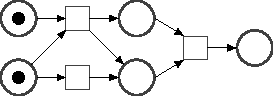
\includegraphics[width=0.7\linewidth]{img/petri_deadlock.pdf}
	  \caption{a Petri net}
	  \label{fig:petrinet}
	\end{subfigure}
	\begin{subfigure}[t]{.32\textwidth}
	  \centering
	  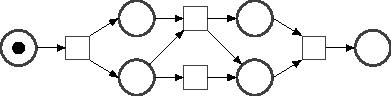
\includegraphics[width=\linewidth]{img/wfnet.pdf}
	  \caption{A workflow net}
	  \label{fig:workflownet}
	\end{subfigure}
	\begin{subfigure}[t]{.32\textwidth}
	  \centering
	  	  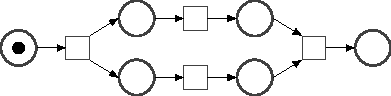
\includegraphics[width=\linewidth]{img/bswfnet.pdf}
	  \caption{A block structured workflow net}
	  \label{fig:blockstructuredworkflownet}
	\end{subfigure}
\caption{Example for petri nets, workflow nets and block structured petri nets. Note that the workflow net does not prevent deadlocks, so it is can't represent a log-based model. The block structured approach on the other hand does prevent deadlocks and is therefore able to represent behavior of traces.}
\label{fig:petri-nets}
\end{figure}
\subsubsection{Directly Follows Graphs}
\begin{wrapfigure}{r}{0.5\textwidth}
	\centering
	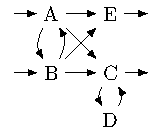
\includegraphics[width=0.25\textwidth]{img/dfgraphExample.pdf}
		\caption{A directly follows graph made from the traces <AE>,<BC>,<ACDC> and <BE>. It captures all follows-realations and the events that are either a first or a last event in a trace.}
		\label{fig:dfgraph}
\end{wrapfigure}
The events in a log are part of ordering relations~\cite{Relations}, e.g. for the trace <ABC> A directly preceeds B and B directly preceeds C. This relation can be expressed via a directly follows graph, that has an edge from node A to node B only if A directly preceeds B at least once in the log.

\subsubsection{Process Trees}
A process tree, defined in ~\cite{ProcessTree}, is a tree-like abstraction of a block structured workflow net. The trees inner nodes represent workflow operators, while the leaves represent events. The basic operators that a process tree supports are $\rightarrow$,$\bigwedge$,$\times$ and $\circlearrowleft$, which correspond to the workflow patterns sequence, parallel split \& join, xor split \& join and cycle defined in ~\cite{workflowpatterns}. Note that $\bigwedge$ and $\times$already include their split and join.\\
Each operator has at least two children which are either events, operators or $\tau$, the silent activity which corresponds to an empty or invisible event.\\
Each operator defines how it's children, denoted as $a_1,...,a_n$ have to be combined as follows:
\begin{labeling}{$\circlearrowleft(a_1,...,a_n)$}
\item [$\rightarrow(a_1,...,a_n)$] - the children are executed from left to right, i.e first $a_1$, then $a_2$ and so on
\item [$\bigwedge(a_1,...,a_n)$] - all children are executed in parallel and intertwined
\item [$\times(a_1,...,a_n)$] - exactly one of the children $a_1,...,a_n$ is executed
\item [$\circlearrowleft(a_1,...,a_n)$] - first $a_1$ is executed, then one of $a_2,...a_n$ followed by $a_1$ may be be executed. The execution of one of $a_2,...a_n$ followed by $a_1$ may repeat.
\end{labeling}
Process trees can easily be converted into other model languages.
\ref{fig:processtree_petrinet} shows a process tree and the corresponding block-structured petri-net.
\begin{figure}[h]
	\begin{subfigure}[t]{.5\textwidth}
	  \centering
	  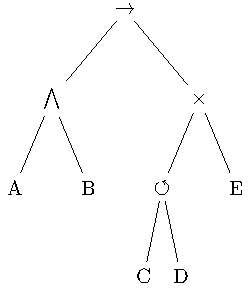
\includegraphics[width=0.5\linewidth]{img/process-tree.pdf}
	  \caption{a Process Tree}
	  \label{fig:process_tree}
	\end{subfigure}
	\begin{subfigure}[t]{.5\textwidth}
	  \centering
	  	  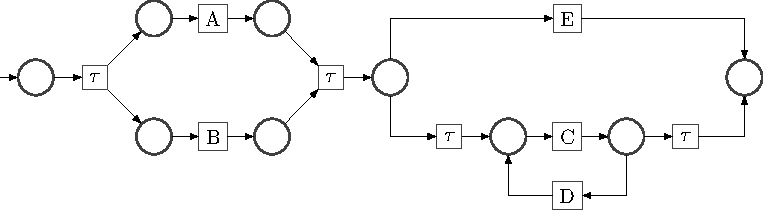
\includegraphics[width=0.9\linewidth]{img/petri-net.pdf}
	  \caption{a Petri Net}
	  \label{fig:petri_net}
	\end{subfigure}
\caption{A process tree and the corresponding block structured petri net. Note that every operator in the process tree is a block in the petri net. $\tau$ is the silent transition that is not seen in a log. It bounds loop- and and-blocks to ensure correct behavior.}
\label{fig:processtree_petrinet}
\end{figure}

\subsubsection{Quality of a Model}
If a model has been discovered an important question is how good the algorithm fares in comparison to others. For this four quality criteria are used that describe different properties of the model the algorithm discovers:
\begin{labeling}{Generalization}
\item [Fitness] Fitness describes to what extend the discovered model is able to replay the traces in the log
\item [Simplicity] Ideally an algorithm should produce simple models. Complex models may be correct, but hard to analyze
\item [Precision] While it is important that a model can produce all behavior in the log, it should not be able to replay too much additional behaviour. Precision captures this aspect. A model that can replay all behavior possible is fit but does not have any value for analysis.
\item [Generalization] Generalization depicts a models ability to reproduce future behavior, i.e. behavior that has not been seen but that will eventually happen.
\end{labeling}

The different criteria contradict themself partially. A precise model may not be a good generalization, while a fit model may not be precise. Different ways to measure these criteria have been proposed, e.g. for measuring fitness some different methods have been proposed in ~\cite{Quality}, ~\cite{Fitnes2} or ~\cite{UsedFitnes}.

\subsection{Types of Process Discovery Algorithms}
~\cite{miningalgorithms} gives an overview of process discovery algorithms that mine petri nets by dividing them into five categories and explaining the shortcomings or benefits of the categories as follows:
\begin{labeling}{Language-Based Region Algorithms}
\item [Abstraction-Based]these algorithms first abstract the log by finding ordering relations between events and then construct a model based on these relations. The $\alpha$-algorithm~\cite{Relations} and it's extensions are the most prominent algorithms of this class
\item[Heuristic-Based]heuristics-based algorithms take into account how frequent behaviour is in the log and are able to filter out low-frequent behavior, called noise, and create a model that represents the main behavior of the log. This is in contrast to abstraction-based algorithms who incorporate all behavior of the log into the final model. Heuristics Miner~\cite{HeuristicsMiner} is an example of such an algorithm
\item[Search-Based]heuristics-based algorithms work on local information of the log, e.g. directly follows-relations and frequencies of these relations, but some workflow constructs are dependent on global information that is not accessible via direct relationships between events. Algorithms like proposed in ~\cite{GeneticMiner} use genetic evolution of a population of models to find the most fitting model for the log. These genetic approaches generate a model and check how well it can parse the traces in the log and evolve the models that are able to reproduce the bahviour of the log the closest. As this procedure has to generate and test models multiple times it's runtime is usually higher than that of other methods
\item[Language-Based Region Algorithms]such algorithms that view a log as a bag of words and that try to generate a model by using language-based region theory like in  ~\cite{LanguageMiner} are called language-based
\item[State Discovery Algorithms]state discovery algorithms view each trace in a log as a transition system. All of these systems are then combined into a single transition system which is then converted into a petri net, like described in ~\cite{StateMiner}
\end{labeling}
On the problem of scalability many proposals have been made. ~\cite{MapReduce} uses MapReduce to make specification mining algorithms more scalable. ~\cite{Passages} partitions the traces passages, which are sets of events X and Y for which X always preceeds Y and Y always follows X. These passages can be analyzed independently.\\
For algorithms that use the theory of region to discover a model the main bottleneck is memory consumption. ~\cite{Regions} tries to minimize this bottleneck by splitting the input, analyzing each subset and combining the analyzed parts again.
\subsection{Inductive Miner and Inductive Miner infrequent}
\paragraph*{Inductive Miner}
Many abstraction-based algorithms are not able to rediscover models that are sound and fitting in finite time, e.g. the alpha-algorithm is not able to discover short loops and produces an unsound model, i.e. models containing deadlocks.\\ 
As a solution Inductive Miner~\cite{InductiveMiner} has been proposed. Inductive Miner is an abstraction-based process discovery algorithm that uses a divide-and-conquer-approach to discover a process tree. The algorithm is able to rediscover a sound and fitting model in finite time.\\\\
To do so, first the algorithm transforms the log $L$ into a directly follows-graph $G(L)$. After creating the directly follows graph the algorithm tries to partition the graph $G(L)$ into smaller subsets $\Sigma_1,...,\Sigma_n$ by finding the dominant workflow operator between the partitions.\\
This dominant workflow operator can be expressed as a cut of the graph $\bigoplus(\Sigma_1,...,\Sigma_n)$, which is an operator that describes how the subsets would have to be combined in order to reproduce the original graph, i.e. for which $\bigoplus(\Sigma_1,...,\Sigma_n)=G(L)$ holds true. \\\\The 4 cut types that have been defined are $\rightarrow$,$\bigwedge$,$\times$ and $\circlearrowleft$, which are exactly the operators that a process tree uses for it's inner nodes.\\
If the dominant cut of a directly follows-graph is a sequence-cut ($\rightarrow(\Sigma_1,...,\Sigma_n)$), then for any node $a\in\Sigma_i$ and $b\in\Sigma_j$ for $i<j$ there is a path from $a$ to $b$ but not the other way around.\\ For a xor-cut ($\times(\Sigma_1,...,\Sigma_n)$) there is no edge between any two nodes $a\in\Sigma_i$ and $b\in\Sigma_j$ for which $i\neq j$. \\
In the case of ($\bigwedge(\Sigma_1,...,\Sigma_n)$), an and-cut, there is a path between any two nodes $a\in\Sigma_i$ and $b\in\Sigma_j$ for which $i\neq j$ and for loop-cuts ($\circlearrowleft(\Sigma_1,...,\Sigma_n)$) all start and ending-nodes are in $\Sigma_1$ while for all $\Sigma_i$ with $i>1$ incoming edges come from an ending node of $\Sigma_1$ and outgoing edges go to a starting node of $\Sigma_1$. \ref{fig:netClasses} visualizes the four cuts.\\
\begin{figure}[h]
	\begin{subfigure}[t]{.5\textwidth}
	  \centering
	  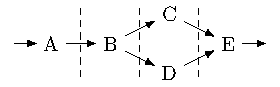
\includegraphics[width=\linewidth]{img/seq_cut.pdf}
	  \caption{A sequence cut. The arrows cross the cut lines only in one direction and an ordering sections is visible. The $\Sigma$ are ${A},{B},{C,D}$ and ${E}$}
	  \label{fig:seq_cut}
	\end{subfigure}
	\begin{subfigure}[t]{.5\textwidth}
		\centering
			  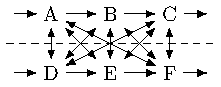
\includegraphics[width=0.8\linewidth]{img/and_cut.pdf}
			  \caption{An and cut. There is an edge between any nodes that are in different $\Sigma$. The $\Sigma$ are ${A,B,C}$ and ${E,F,G}$}
			  \label{fig:and_cut}
	\end{subfigure}
	\begin{subfigure}[t]{.5\textwidth}
		\centering
			  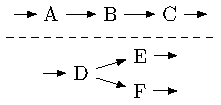
\includegraphics[width=0.8\linewidth]{img/xor_cut.pdf}
			  \caption{A xor cut. Each $\Sigma$ is a single connected component of the graph. The $\Sigma$ are ${A,B,C}$ and ${D,E,F}$}
			  \label{fig:xor_cut}
	\end{subfigure}
		\begin{subfigure}[t]{.5\textwidth}
			\centering
				  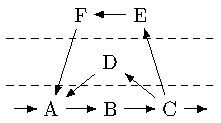
\includegraphics[width=0.8\linewidth]{img/loop_cut.pdf}
				  \caption{A loop cut. $\Sigma_1$ has all starting- and end-nodes while all other $\Sigma$ have incoming edges from an ending node of $\Sigma_1$ and outgoing edges to a startinhow they appear ing node of $\Sigma_1$. The $\Sigma$ are ${A,B,C}$,${D}$ and ${E,F}$.}
				  \label{fig:loop_cut}
		\end{subfigure}
\caption{The different cut types how they appear in the df-graph. Dashed lines denote cuts.}
\label{fig:netClasses}
\end{figure}
Should the algorithm not be able to find a cut on a given graph, then it returns a flower model $\circlearrowleft(\tau, a_1,...,a_n)$ for which $a_1,...,a_n$ are the events that are part of $G(L)$.\\
With the chosen cut we can construct a node in the process tree. Assume we have G(L) and the chosen cut is $\circlearrowleft(\Sigma_1,...,\Sigma_n)$, then $\circlearrowleft$ is the process tree operator and it's children are the results of the recursively analyzed $\Sigma_1,...,\Sigma_n$.\\\\ See \ref{fig:IM} for an example of how Inductive Miner transforms a directly follows graph into a process-tree.
\begin{figure}
\begin{subfigure}[t]{\textwidth}
 \begin{subfigure}[t]{0.5\textwidth}
 \centering
 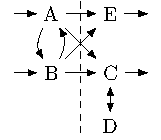
\includegraphics[width=0.5\linewidth]{img/IMExample_initial.pdf}
 \end{subfigure}
 \begin{subfigure}[t]{0.5\textwidth}
  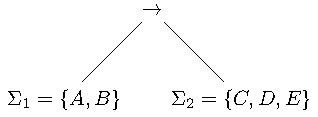
\includegraphics[width=0.9\linewidth]{img/sequence_tree.pdf}
 \end{subfigure}
 \caption{The first detected cut is a sequence cut. The operator is added as the root node and the algorithm recurses on the partitions.}
\end{subfigure}
\begin{subfigure}[t]{\textwidth}
 \begin{subfigure}[t]{0.5\textwidth}
  \centering
  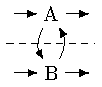
\includegraphics[width=0.3\linewidth]{img/IMExample_and.pdf}
 \end{subfigure}
 \begin{subfigure}[t]{0.5\textwidth}
   \centering
   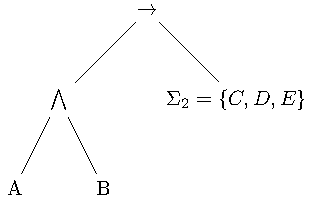
\includegraphics[width=0.5\linewidth]{img/and_tree.pdf}
 \end{subfigure}
  \caption{The algorithm detects an and cut and recurses on $\Sigma_1\{A\}$ and $\Sigma_2\{B\}$. As the two partitions are base cases the event is returned and appended as a leaf node.}
\end{subfigure}
\begin{subfigure}[t]{\textwidth}
 \begin{subfigure}[t]{0.5\textwidth}
   \centering
   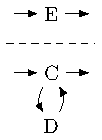
\includegraphics[width=0.3\linewidth]{img/IMExample_xor.pdf}
 \end{subfigure}
 \begin{subfigure}[t]{0.5\textwidth}
   \centering
   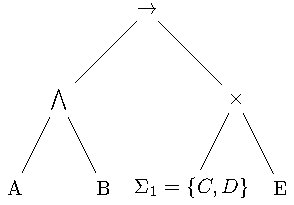
\includegraphics[width=0.5\linewidth]{img/xor_tree.pdf}
 \end{subfigure}
    \caption{In the next step an xor cut is detected. Upon recursion of $\Sigma_2$ the single event E is appended as a child.}
\end{subfigure}
\begin{subfigure}[t]{\textwidth}
 \begin{subfigure}[t]{0.5\textwidth}
    \centering
    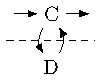
\includegraphics[width=0.3\linewidth]{img/IMExample_final.pdf}
 \end{subfigure}
 \begin{subfigure}[t]{0.5\textwidth}
    \centering
    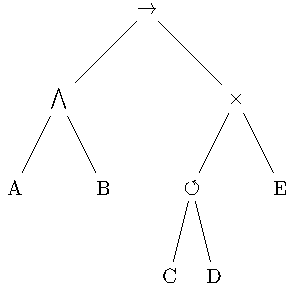
\includegraphics[width=0.5\linewidth]{img/xor_tree_final.pdf}
 \end{subfigure}
     \caption{Lastly a loop cut is detected. The partitions resemble base cases, so they are added as leaves. As there is no further partition that has to be analyzed the algorithm returns the process tree as the discovered model}
\end{subfigure}
\caption{Inductive Miner discovering a model of Log $L=\{<ABCDC>,<BAE>,<BAC>\}$}
\label{fig:IM}
\end{figure}
\paragraph{Inductive Miner infrequent}
Inductive Miner considers all behavior of the log for the discovered model, even behavior that is infrequent or unwanted. In some cases, for example if this infrequent behavior is considered as noise, or if one wants just an overview of the main behavior of the log, then Inductive Miner is not a feasible option.
To allow the usage of Inductive Miner in these use cases Inductive Miner infrequent has been proposed ~\cite{InductiveMinerInfrequent}, a heuristics-based adaption of Inductive Miner that filters infrequent behavior and produces a reduced model, that is not perfectly fit anymore but more concise than a perfectly fit model.
In each recursion step IMi first applies the normal steps that IM would do. If no cut could be applied and a flower model would be returned, it applies filter rules instead.\\\\
In order to do so IMi keeps track of how frequent traces and events are in the log and uses a user-chosen frequency threshold $k$ between 0 and 1. Upon cut detection infrequent edges whose frequencies are lower then k times the frequency of the most frequent edge in the graph are removed. Foror $\rightarrow$ cut detection a modified directly follows graph is used that amplifies the frequencies of frequent edges. This allows for a better distinction between wanted and unwanted behaviour.\\
Furthermore frequency-based filtering rules on base cases are introduced as the application of filter rules may introduce empty traces and repetitions of events in subsets. These rules try to select the most-fitting model for these distorted base cases.\\
Lastly after operator selection filter rules are applied on the partitioned subsets that remove the least operator infringing events from the log, to allow for a clean log for the next recursive step.\\
In evaluations IMi took longer than IM to finish, but was still faster than most other heuristics-based approaches.
\begin{figure}[h]
	\begin{subfigure}[t]{.9\textwidth}
	  \centering
	  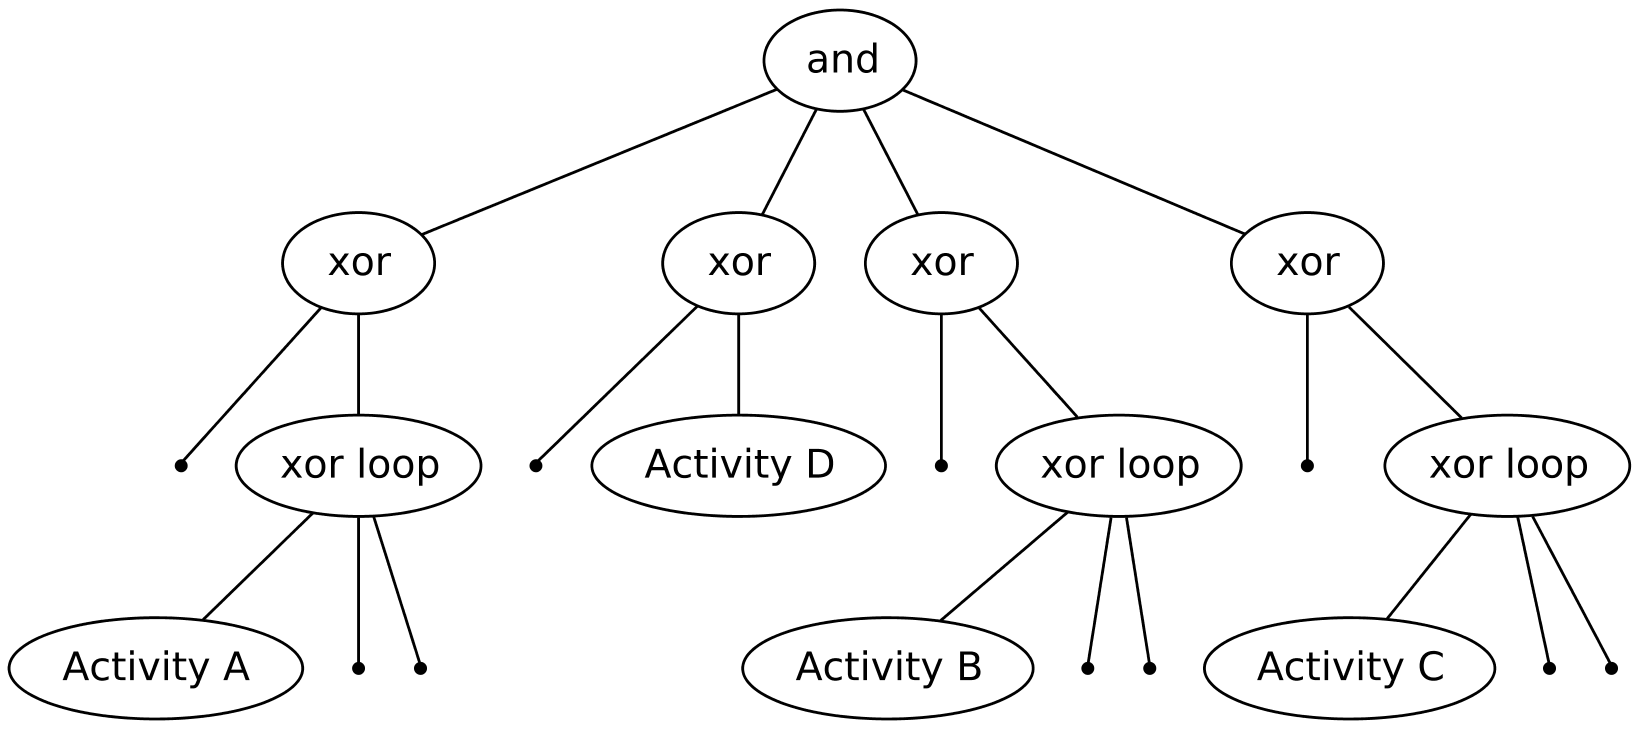
\includegraphics[width=0.5\linewidth]{img/noise.png}
	  \caption{IM discovers a complex tree as each edge is considered.}
	\end{subfigure}
	\begin{subfigure}[t]{.9\textwidth}
	  \centering
	  	  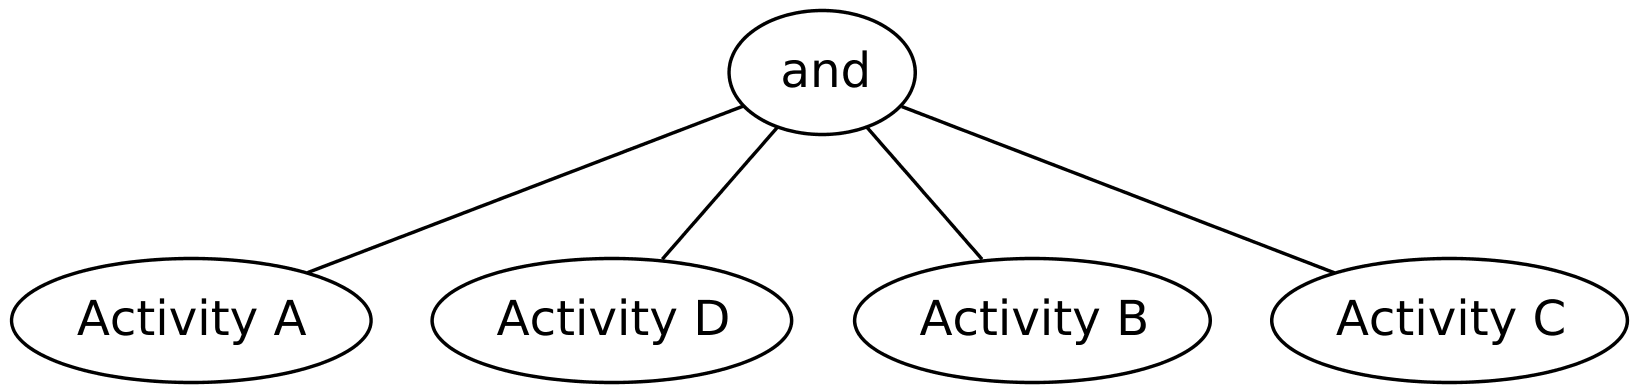
\includegraphics[width=0.45\linewidth]{img/noiseless.png}
	  \caption{IMi is able to correctly discover the sequence.}
	\end{subfigure}
\caption{Models as they are discovered by IM and IMi. The log represents a sequence of 4 events with added noise. IM creates a complex model while IMi discovers just the main behavior.}
\label{fig:IMvsIMi}
\end{figure}

\subsection{Incremental Process Discovery}
Most Process Discovery algorithms base their analysis on the whole input log. Heuristics-based algorithms try to ignore infrequent bahaviour but still base their analysis on all traces. In a real-life scenario a log usually contains highly redundant information, either because some few processes are dominant in the log or because the underlying process only allows for so much behavior. Therefore it would be a good idea to not consider the whole log $L$ but only a subset $L_{min}\subset L$ that contains the minimum information to discover the correct model. Stream-based discovery algorithms~\cite{Streams} have to take a similar approach, as the unbound size of log streams and the main memory boundary only allow for a window of traces, usually the newest ones, that can be considered for a representative model.\\\\
~\cite{PartialLogAnalysis} proposes a statistical method that considers only a sublog of L based on the estimated probability $p^{}$ of new traces containing new information given a set of traces that have already been seen.\\
In the work the approach has been evaluated based on the k-tails algorithm~\cite{KTails} that uses k-sequences, sequences of consecutive events in the log.\\\\
The author defined the notion of $\delta$-similarity as a criteria that tells when "enough" information has been seen and when the analysis can be stopped. A log $L$ is $\delta$-similar if the total probability of k-sequences to be observed in the next trace that would be seen in the next trace is smaller than $\delta$.\\ In order to precisely estimate $\delta$ one would have to know in advance how many k-sequences are remaining in the following traces at any given time. In a real scenario this is not reasonable as one would need to analyze the log in advance which destroys the purpose of the algorithm, which is not to consider everything for the discovery. One can not know the exact value of $\delta$ but one can try to estimate it using interval estimation methods by modeling the process of iteratively selecting a trace and checking whether it contains new information or not as a series of binomial experiments. With this view one can calculate the number of consecutive experiments that have to fail in order to safely conclude that no new information is expected in the remaining log.\\\\
By simulating a series of iterations in which one checks whether new information is seen or not the propbability $p$ can be bound inside a binomial proportions interval with upper and lower bound $p^{}_{lower bound}$ and $p^{}_{upper bound}$.\\
Let $p^{}$ be the proportion of succesful trials over N random trials and let z be the $1-0,5\cdot \alpha$ percentile of a normal distribution for a given $\alpha$, then the binomial proportions interval
\begin{align*}
[\frac{1}{1+\frac{z^2}{N}}\cdot(p^{}+\frac{z^2}{2N}-\sqrt{\frac{p^{}\cdot(1-p^{})}{N}+\frac{z}{4N^2}}),\frac{1}{1+\frac{z^2}{N}}\cdot(p^{}+\frac{z^2}{2N}+\sqrt{\frac{p^{}\cdot(1-p^{})}{N}+\frac{z}{4N^2}})]
\end{align*}
contains the real value p with a probability of $(1-\alpha)$. The used formula is Wilson's interval. Alternatively the paper cited Agresti-Coull interval or Jeffreys prior intervall as superior interval methods for different $p$~\cite{Intervals}.\\\\
Now one simply have to calculate how many failing trials N are needed until $p^{}_{upper bound}<\delta$. Upon finding an N one knows that consecutive traces without new information are needed to conclude with a $(1-\alpha)$ confidence that the log is is $\delta$-similar. As one wants to simulate all tests to fail $1-p^{}$ will be set to $0$, thus reducing the formula to
\begin{align*}
\frac{1}{1+\frac{z^2}{N}}\cdot(\frac{z^2}{2\cdot N}+\sqrt{\frac{z}{4\cdot N^2}})
\end{align*}
For $\alpha=0.01$ and $\delta=0.05$ this would give $N=128$ using the above formula. Thus after seeing 128 traces that do not contain new information one can stop the analysis knowing with a confidence of $0.99$ that the probability of seeing new information is less than $\delta$.\\
One can calculate N before applying the algorithm . Then while analyzing traces one just has to keep track of the amount of consecutive traces without new information and stop the analysis after N consecute traces have been seen that yielded no new information.\\
\section{The statistical Inductive Miner}
\subsection{Idea}
Assume a user wants to get a general overwiev of the behavior in a log. The user also wants to measure the average cycle time of the model.\\
For this use case the Inductive Miner infrequent is an ideal choice.
\\\\
In ~\cite{PartialLogAnalysis} it was shown that the statisticallLog analysis is independent on the discovery algorithm it is used for, one only needs to know whether new information has been gained through a trace or not. Consequently one should be able to adapt the information detection so that it is usebale for a specific algorithm, then mine the reduced sublog and still discover a fitting model. If the log processing considers all trace properties that could change the underlying model representation, then the statistical pre-processing step should produce a sublog, that contains all relevant information for the algorithm.\\\\
If IMi is executed with a Log that has been pre-processed with criteria that are relevant for Inductive Miner, the runtime and memory consumption of the algorithm could be reduced and in turn enable the analysis of bigger data.\\
\subsection{Algorithm}
A statistical pre-processing step is added to IM, in which N is calculated, the number of consecutive traces without new information that have to be read to end the trace collection, then the algorithmg chooses random traces repeadedly, checks for new information in the chosen trace and increments a counter if no new information has been seen, or resets it to 0 otherwise. If the counter has reached N, the traces seen up to tis point form the new log for which IMi will discover a model. See Figure~\ref{fig:algorithm} for a visualization of the algorithmic setup.\\
\begin{figure}[h]
	\caption{The Algorithm}
	\label{fig:algorithm}
	\includegraphics[width=\linewidth]{Algorithm.png}
\end{figure}
As IM is already implemented in ProM~\cite{ProM} a statistical pre-processing framework is added that takes a log $L$ and that returns a log $L_{new}\subseteq L$ and calls the already implemented IM with $L_{new}$. This will be slower than using the information extraction step that IM will do when it is called but allows to completely ignore the implementation details of IM.\\
For the trace calculation any of the binomial proportion interval estimators is used. N is incremented repeadedly until the estimated upper bound of $p$ is lower than $\delta$.\\
\subsection{The Information Detection Framework of sIMi}
\subsubsection{Defining a general Information Detection Framework}
The general idea presented in ~\cite{PartialLogAnalysis} is to choose a random trace from the log and analyse whether this log contains any new information that change the inner representation of the log. If so, then the experimental chain starts again, otherwise it continues with the next randomly chosen trace until the threshold has been reached the complete log has been traversed.\\ 
For k-Tails the inner representation is the set of n-grams or k-tails seen so far. If a trace adds a new n-gram then the representation changes.\\\\
Having this general idea in mind one can formalize a general algorithm-independent framework $F$ that detects new information in traces as follows:\\
Given a set of informations aspects $I_1,...,I_n$, then each aspect has a corresponding information base, denoted as $B_{I_1},...,B_{I_n}$ that holds all information extracted from traces so far. Furthermore for every $I_j$ there exists a function $DETECT_{I_j}(B_{I_j}, t)$, that, based on the current trace $t$ and $B_{I_j}$, returns whether the traces yields new information for $I_j$ or not.\\
Thus for information bases $B_{I_1},...,B_{I_n}$ and a trace $t$ the function
\begin{align*}
G = DETECT_{I_1}(B_{I_1},t) \vee DETECT_{I_2}(B_{I_2},t) \vee ... \vee DETECT_{I_n}(B_{I_n},t)
\end{align*}
calcaulates whether $t$ contains new information or not.\\
In the case of k-tails the framework $F_{k-tails}$ would contain
\begin{labeling}{$DETECT_{I_{n-gram}}(B_{I_{n-gram}},t)$}
	\item[$I_{n-gram}$] n-grams seen in the traces
	\item[$B_{I_{n-gram}}$] a data structure, that contains the seen n-grams
	\item[$DETECT_{I_{n-gram}}(B_{I_{n-gram}},t)$] the function that for a given trace $t$ returns whether $t$ contains a n-gram that is not yet present in $B_{I_1}$ and updates $B_{I_1}$ with new n-grams
\end{labeling}
\subsubsection{Notable properties of the Framework}
Just from this setup one can conclude several properties of the framework:
\paragraph{Trace order dependent information detection}
Let $t_current$ denote the current trace, then $t_{current\pm i}$ denotes the trace that has been analyzed i steps prior or after $t_current$ .\\
Whether $F_{I_j}$ yields new information or not is highly dependent on the state of $B_{I_j}$ while analyzing $t_current$. Depending on the order of chosen traces a trace could yield new information or not, e.g. if $<ABC>,<ABE>$ have been analyzed prior to the trace $<AB>$, then $<AB>$ does not contain new information, whereas in an other scenario it would contain new information.\\\\The analysis of the first trace will always yield new information.
\paragraph{Extensibility of the framework}
The framework does give constraints on neither the type of information that will be analyzed, nor the amount of criteria that will be analyzed.\\ As such a user may add or remove analytical criteria as he sees fit. Removing an aspect will not affect the outcome of other aspects if they do not depend on the information base of the removed aspect.
\paragraph{Ordering of aspects}
As the $DETECT$-functions are only dependent on $B_{I_j}$ they can be executed in any order.
\paragraph{Aspect dependent runtime}
Some information aspects see new information more frequently than others, some will also get more information out of a trace than others. Assuming that all but one aspect won't get any new information out of the log, but the remaining aspect still gets new information through the analysis of following traces, then this aspect prolongs the log preprocessing single handedly. The preprocessingwill only stop, when this remaining aspect does not gain new information anymore. One can say that this information aspect determines the total runtime of the preprocessing framework.\\ 
\paragraph{Aspect dependent reliability}
For each trace each $I_j$ is analyzed.\\ The more $I_j$ are present, the higher is the chance that $t_current$ will yield new information. Assuming that the order of $t_current,t_{current+1},...,t_{current+1},$ is known in advance, then there could be one ordering of traces for which each consecutive analysis yields no new information and the whole preprocessing chain comes to an end too early.\\
Adding more criteria decreases the chance of this happening and therefore increases the reliability of the framework.
\paragraph{Aspect-based runtime and memory}
The total runtime and memory of analyzing $t_current$ is $\sum_{j=1}^{n} O(B_{I_j})$ and therefore $\max(B_{I_j})$ for $j<n$.
\subsection{Analytical Aspects for sIM}
\subsubsection{Model correctness}
\paragraph{Simulating the directly follows graph during pre processing}
In the case of Inductive Miner a trace $t$ yields new information if the directly-follows graph changed after reading in $t$.
To ensure a correct model with the framework it should therefore be feasible to represent the directly follows graph through all aspects that could change the graph itself. The chosen aspects correspond to the $I_j$ in our framework. By ensuring that we can recronstruct the graph by just using all $B_{I_j}$ we can be sure that all relevant information is captured through our aspects. $DETECT_{I_j}$ detects a change in the graph by detecting a change in $B_{I_j}$, so all it has to do is to check, whether something new has been added to $B_{I_j}$ by $t$ or not.
\paragraph{Using changeable graph properties as analysis aspects}
A directly follows graph is represented through a set of vertices, edges, start- and ending nodes. Given a trace $t$ it may add
\begin{itemize}
\item a single starting node
\item a single ending node
\item multiple new vertices
\item multiple new edges
\end{itemize}
to the graph.
These graph aspects are the $I_j$ for the sIM-framework. \ref{fig:dfgraphchanging} shows that these criteria are able to detect a change in the knowledge base that IM uses. \ref{fig:dfgraphbuilding} further shows that it is possible to rebuild the directly follows graph using just these informations.
\begin{figure}[h]
	\begin{subfigure}[t]{.5\textwidth}
	  \centering
	  %\includegraphics[width=.9\linewidth]{img/dfgraph.pdf}g
	  \caption{A directly follows graph made of the traces <ABD> and <ACE>}
	\end{subfigure}%
	\begin{subfigure}[t]{.45\textwidth}
	  \centering
	  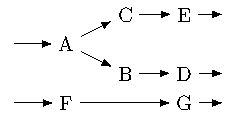
\includegraphics[width=.9\linewidth]{img/dfgraph_added_trace.pdf}
	  \caption{The same graph after <FG> has been added}
	  	\label{fig:dfgraphchangingafter}
	\end{subfigure}
	\caption{Adding the trace <FG> to the initial graph adds a new starting- and end node, two new events and one new edge to the graph}
	\label{fig:dfgraphchanging}
\end{figure}
\begin{figure}[h]
	\begin{subfigure}[t]{.32\textwidth}
	  \centering
	  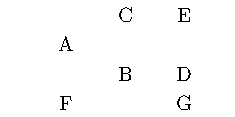
\includegraphics[width=.9\linewidth]{img/nodes.pdf}
	  \caption{Adding nodes}
	\end{subfigure}%
	\begin{subfigure}[t]{.32\textwidth}
	  \centering
	  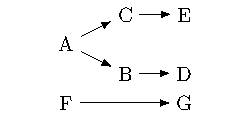
\includegraphics[width=.9\linewidth]{img/nodes_edges.pdf}
	  \caption{Adding edges}
	\end{subfigure}
	\begin{subfigure}[t]{.32\textwidth}
	  \centering
	  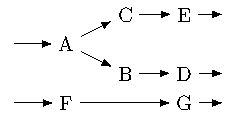
\includegraphics[width=.9\linewidth]{img/nodes_start_end_edges.pdf}
	  \caption{Adding starting- and end nodes}
	\end{subfigure}
	\caption{Reconstructing the directly follows graph from \ref{fig:dfgraphchangingafter} by using the information seen in the traces.}
	\label{fig:dfgraphbuilding}
\end{figure}
\subsubsection{Cycle Time Correctness}
For model criteria a trace $t$ yields new information if after reading the trace the corresponding knowledge base has changed.\\ For cycle times almost every trace will change the knowledge base, because every trace contains a cycle time and a small difference from the estimated cycle time will change the value of the new updated cycle time. Every cycle time but the one that is equals to the cycle time measured so far would yield new information. If this strict change would be used as $DETECT_{cycle time}$ then most likely all traces would have to be considered for the pre-processing step, making the whole framework too restrictive, making it slower than IMi.\\
If one regards the calculated cycle times after each trace as a sequence of values, then onw can see that the sequence converges towards the correct average cycle time.\\
Let $t_n$, $t_m$ denote the n'th and m'th trace that will be analyzed, $|t|$ the index of trace $t$ in the sequence, and $cycle time_n$,$cycle time_m$ the estimated cycle time at $t_n$ and $t_m$. Furthermore $d(cycle time_n, cycle time_m):=|cycle time_n - cycle time_m|$ is the function that calculates the distance between two cycle times. As this sequence converges and the space of possible cycle times is a complete metric space, it follows that the sequence is a Cauchy-sequence and therefore
\begin{align*}
\forall \epsilon\geq0 \exists 0<N<\max(|t|) \forall N\leq t_n,t_m <\max(|t|): d(cycle time_n, cycle time_m)<\epsilon
\end{align*}
holds true.\\
No matter what sequence of cycle times one has, for a given analysis one can choose an arbitrary $\epsilon$ and know that after an unknown number of traces n $d(cycle time_n, cycle time_{n+1})$ will be smaller than $\epsilon$ for every $m\geq n$.\\
Knowing this  the correct cycle time can be approximated by choosing an $\epsilon$ and checking whether $d(cycle time_{n-1}, cycle time_n)\geq \epsilon$ is true or not. If it is true then that trace is treated as if it yields new information for $I_{cycle time}$.\\\\
\paragraph{Model based and Event based cycle time approximation} There are multiple possibilities to approximate the average cycle time of a log. For a trace $t$ one solution is to calculate the time of the trace by either getting it from it's information or calculating it manually by subtracting the beginning time of the first event from the completion time of the last event, updating the average cycle time of the model with the so calculated trace time and testing for $d(cycle time_{n-1}, cycle time_n)\geq \epsilon$.\\
The other possibility is to calculate the completion time of each event in t, updating the average cycle time for each event in the trace and then for each of them checking for the outcome of $d(cycle time_{n-1}, cycle time_n)\geq \epsilon$.\\
Both variants base their calculations on the timestamps present in the log, so two possible functions $DETECT_{cycle time_{model}}$ and $DETECT_{cycle time_{event}}$ exist, that could be used for $I_{cycle time}$.
The second option needs more computation as it may has to do multiple calculations, first option needs to update a single value.
\paragraph{Finding an appropriate $\epsilon$}
The outcome of $DETECT_{cycle time}$ is dependent on the chosen $\epsilon$. It could be chosen so that the event time is approximated in the least traces as possible by setting it high. This would lower the amount of traces that have to be read for the experiment but results in an inaccurate estimated cycle time. If it is chosen to be small, then this increases the number of traces that have to be read during preprocessing but returns a more accurate result. Furthermore choosing an $\epsilon$ that is too small will result in almost every trace yielding new information. In such a case the whole log will be pre-processed and no speed gain is possible. On the other side, if $\epsilon$ is choosen too high, then almost no trace will yield new information, which means that the cycle time analysis does not provide meaningful results and is negligible. In this case one could remove the cycle time analysis as it's only accomplishment would be to slow down the general speed of the algorithm. The chosen $\epsilon$ is highly dependent on the distribution of times in the log. If all events have the same duration, then an event based analysis would finish after if has seen all events once. If all traces have the same duration, then a model based analysis would finish after one trace. How randomly the durations are determines what an appropriate $\epsilon$ may be. Therefore a user has to choose a fitting $\epsilon$ for each log based on the knowledge he or her has about the time distribution.\\\\ Even though the model based cycle time calculation does more work a user may only be able to quantify an appropriate $\epsilon$ for the events in the log, so it may be a good idea to give both options.
\subsubsection{Summarizing all Aspects}
Knowing that we want to guarantee a correct model and a approximately correct average cycle time following components for $F_{sIMi}$ can be defined:
\begin{labeling}{$I_{cycle time_{event}}$}
\item[$I_{event}$] the events seen in the log
\item[$I_{edges}$] the edges seen in the log
\item[$I_{start}$] the starting nodes seen in the log
\item[$I_{ending}$] the end nodes seen in the log
\item[$I_{cycle time_{model}}$] the approximated cycle time based on trace times
\item[$I_{cycle time_{event}}$] the approximated cycle time based on event times
\end{labeling}
\subsection{Infrequent Behaviour}
During the preprocessing the algorithm chooses a random trace for the next analysis.
Assuming that trace $t$ is infrequent in the log, then there are two possible outcomes:
\begin{labeling}{2. $t$ is not chosen}
	\item [2. $t$ is not chosen] then t is not represented in the graph
	\item [1. $t$ is chosen] then t is represented in the directly follows graph but is filtered out by the filtering rules of IMi
\end{labeling}
In both cases $t$ does not have an impact on the mined model.
Traces that appear frequently have a higher chance of being chosen than these that apper infrequently, so sIM can be regarded as a further filter step of IMi and as thus the addition of a statistical preprocessing step to the log should retain the relative frequency of unique traces.
\subsection{Input parameters}
Having defined all of the analysis criteria te input parameters of the algorithm are:
\begin{labeling}{boolean cycle time variant}
	\item [float $\alpha$] - the confidence of the preprocessing
	\item [float $\delta$] - the probability that the estimated $p$ has to reach
	\item [float $\epsilon$] - the epsilon used for the cycle time analysis
	\item [boolean cycle time variant] - 1 if cycle time will be measured on a model basis, 0 if on an event basis
\end{labeling}
\section{Evaluating the Algorithm}
\subsection{Performance Analysis}
\subsubsection{Used Logs}
In order to measure how well the constructed algorithm fares compared to IMi measurements with 2 real life Logs have been performed. All of them were part of the BPI Challenge conducted by the International Workshop on Business Process Intelligence each year~\cite{bpi}. These logs are provided freely for anyone to use as they see fit and will be denoted as follows:
\begin{itemize}
\item[BPI2012] - a log by a dutch financial institute. It contains roughly 13000 traces and is 74.1MB big 
\item[BPI2014] - a log containing incident activity records of a bank of size 39.2MB
\end{itemize}
For each log runtime, memory consumption the number of traces that have been read and the fitness~\cite{UsedFitnes} with regards to the original model have been measured. All measurements have been conducted with varying $\epsilon$ on model and event view. $\alpha$ has been set to 0.01 and $\delta$ to 0.99. Wilson interval is used as the interval estimator. This sets the number of traces that have to be read to 127.\\
The chosen $\epsilon$ differs for all logs because approriate values for $\epsilon$ are dependant on the distribuion of trace and event times in the log.
\subsubsection{Runtime}
\begin{figure}[h]
	\begin{subfigure}{.5\textwidth}
	  \centering
	  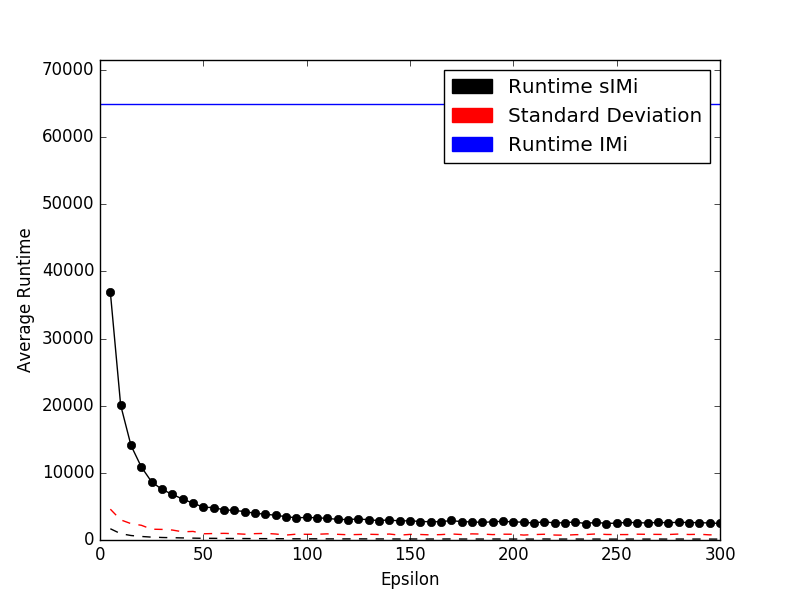
\includegraphics[width=.9\linewidth]{data/BPI2012/BPI_2012_lax_threshold_time.png}
	  \caption{BPI2012}
	  \label{fig:runtime12}
	\end{subfigure}%
	\begin{subfigure}{.5\textwidth}
	  \centering
	  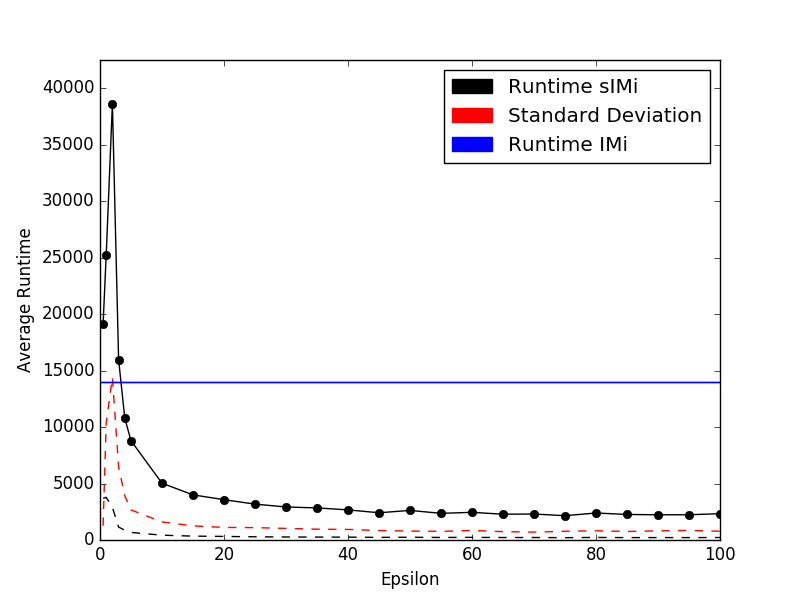
\includegraphics[width=.9\linewidth]{data/BPI2014/BPI2014_lax_threshold_timeAllData.png}
	  \caption{BPI2014}
	  \label{fig:runtime14}
	\end{subfigure}
	\caption{Average totalrRuntime (black continous) and average preprocessing time (black dotted) with varying $\epsilon$, model-based}
	\label{fig:runtime1214}
\end{figure}
As shown in \ref{fig:runtime1214} sIMi is notably faster for most $epsilon$, for BPI2012 it produces a model 20 times faster than IMi for big $\epsilon$. For BPI2014 the model can be produced up to 5 times as fast with preprocseeing being only a fraction of the total time. The impact on the chosen $\epsilon$ on the total runtime is very immense for small $\epsilon$ as then the cycle time analysis becomes the most restrictive information aspect during preprocessing.\\
For a small window of $\epsilon$ (for BPI2014 approximately $0.5m<\epsilon<2$m) the runtime is notably higher than the runtime of IMi though. This is because the logs get partially ordered when they are importet into ProM, but the algorithm builds the new log randomly. As the implementation of IMi benefits from an ordered log the traces of the new log are ordered in the same way they are in the original log, so that the total runtime in cases where a large portion of the log gets seen is higher than IMi. Therefore we can say that sIMi is faster than IMi apart from cases where $\epsilon$ is very small.\\
One can clearly see that an $\epsilon$ that is choosen too high will not have any impact on the runtime. This is due to the cycle time analysis finishing much faster than at least one of the model based information aspects, which then determines the runtime. For BPI2012 this seems to be the case for $epsilon>150m$, for BPI2014 $\epsilon>40m$.\\
Because of the higher amount of traces that have to be read for small $\epsilon$ and because the cycle time analysis is the only information aspect that prolongs the preprocessing in these cases the fluctuation of runtimes grows bigger, which can be seen in the standard deviation of the estimated runtimes that rises sharply for small $\epsilon$. This leads to the assumption that the pre processing becomes unstable in cases where the cycle time is the most restrictive information aspect and where not all traces are seen.\\
If one compares runtimes for different $\epsilon$ like in \ref{fig:runtimeMeasurements1214} then one can see that the runtimes gets indeed more unstable for small $\epsilon$, so differing runtimes are expected for small $\epsilon$.\\
\begin{figure}[h]
	\begin{subfigure}{.5\textwidth}
	  \centering
	  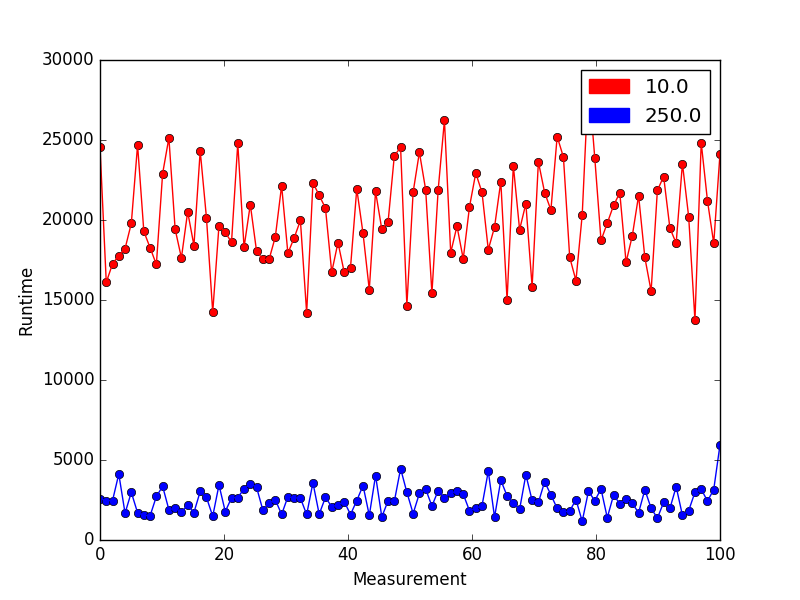
\includegraphics[width=.9\linewidth]{data/BPI2012/lax_10_250_runtime.png}
	  \caption{BPI2012 }
	  \label{fig:runtimeMeasurement12}
	\end{subfigure}%
	\begin{subfigure}{.5\textwidth}
	  \centering
	  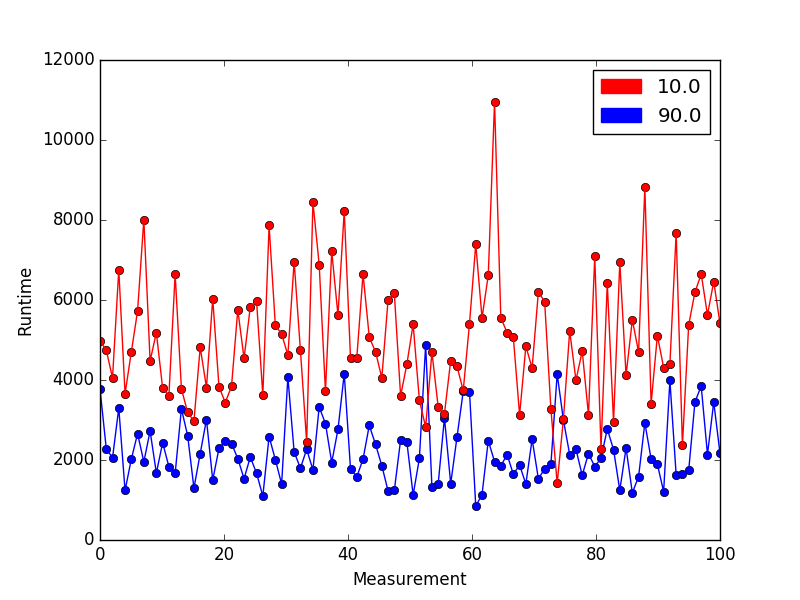
\includegraphics[width=.9\linewidth]{data/BPI2014/lax_10_90_runtime.png}
	  \caption{BPI2014}
	  \label{fig:runtimeMeasurement14}
	\end{subfigure}
	\caption{Comparison 100 measured runtimes for BPI2012 and BPI2014 using two different $\epsilon$, model-based}
	\label{fig:runtimeMeasurements1214}
\end{figure}
\subsubsection{Traces}
\begin{figure}[h]
	\begin{subfigure}{.5\textwidth}
	  \centering
	  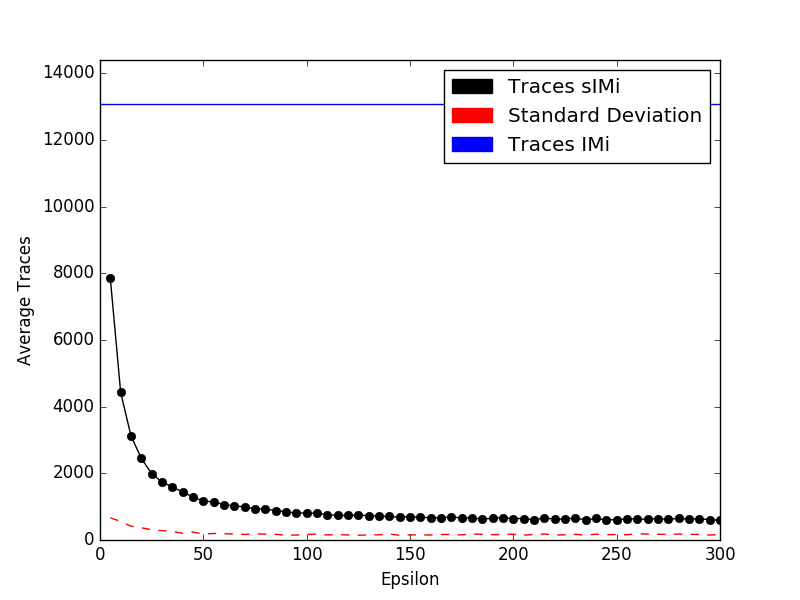
\includegraphics[width=.9\linewidth]{data/BPI2012/BPI_2012_lax_threshold_traces.png}
	  \caption{BPI2012}
	  \label{fig:traces12}
	\end{subfigure}%
	\begin{subfigure}{.5\textwidth}
	  \centering
	  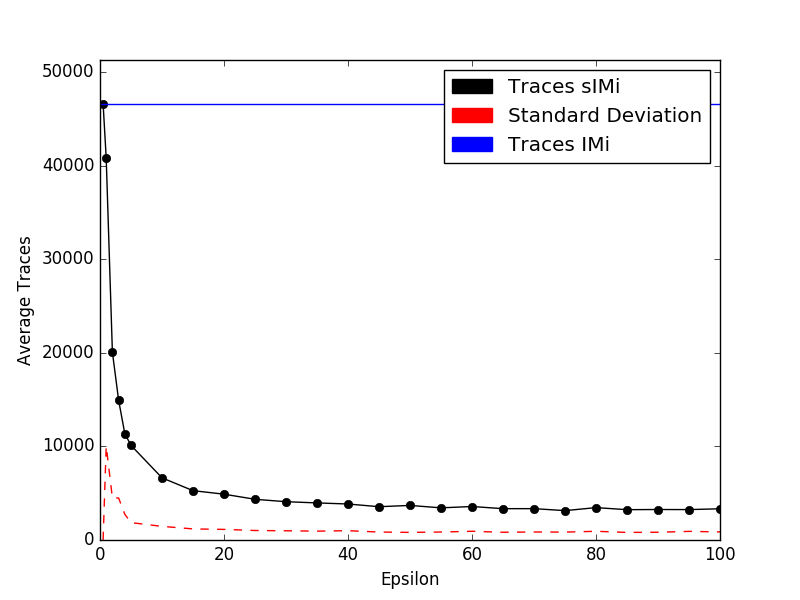
\includegraphics[width=.9\linewidth]{data/BPI2014/BPI2014_lax_threshold_traces.png}
	  \caption{BPI2014}
	  \label{fig:traces14}
	\end{subfigure}
	\caption{Average number of traces per run with varying $\epsilon$, model-based}
	\label{fig:traces1214}
\end{figure}
As the runtime is completely dependent on the number of traces that are seen in a run of the algorithm we can assume that the number of traces the algorithm has to read develops roughly the same for verying $\epsilon$, which means that
\begin{itemize}
\item for small $\epsilon$ the number of traces rises sharply until the total log size is reached
\item for big $\epsilon$ the number of traces will stay roughly the same
\end{itemize}
\subsubsection{Memory}
\begin{figure}[h]
	\begin{subfigure}{.5\textwidth}
	  \centering
	  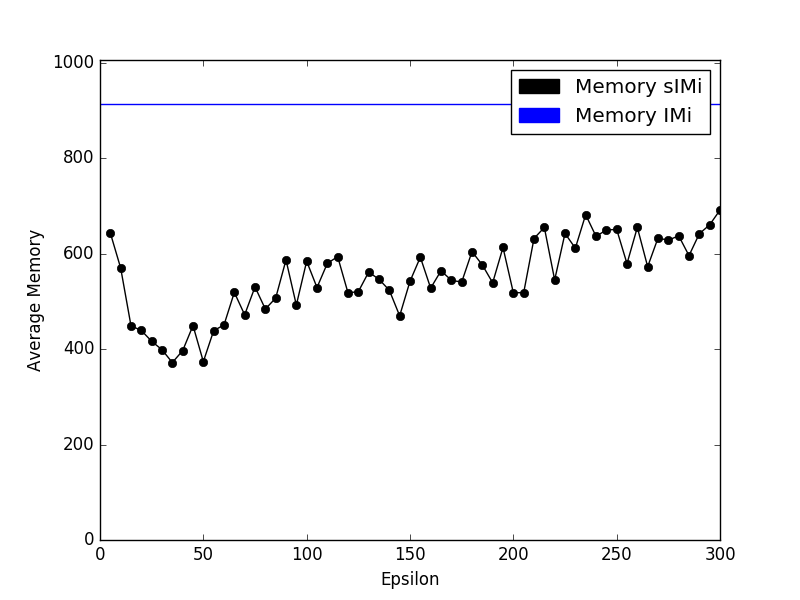
\includegraphics[width=.9\linewidth]{data/BPI2012/BPI_2012_lax_threshold_memory.png}
	  \caption{BPI2012}
	  \label{fig:mem12}
	\end{subfigure}%
	\begin{subfigure}{.5\textwidth}
	  \centering
	  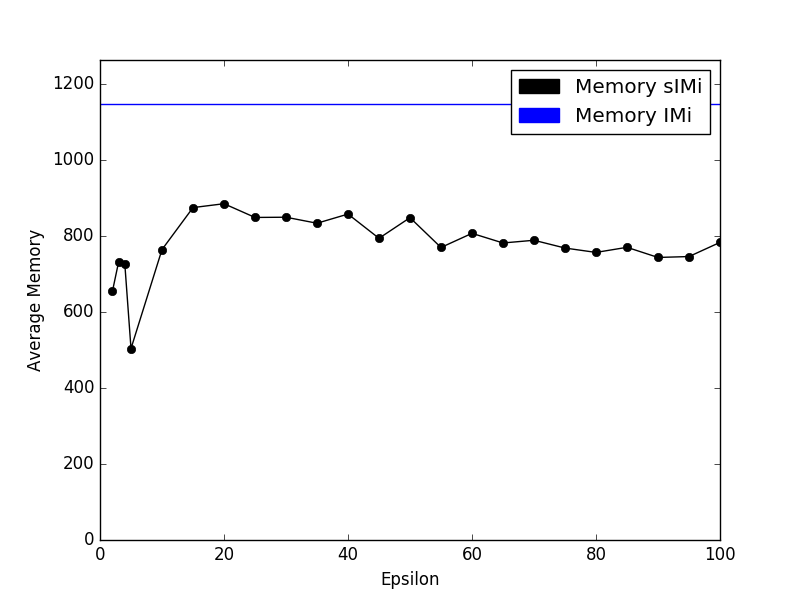
\includegraphics[width=.9\linewidth]{data/BPI2014/BPI2014_lax_threshold_memory.png}
	  \caption{BPI2014}
	  \label{fig:mem14}
	\end{subfigure}
	\caption{Average memory consumption of sIMi with varying $\epsilon$, model-based}
	\label{fig:mem1214}
\end{figure}
Even though runtime and traces are affected by the chosen $\epsilon$ the memory seems not to be influenced by $\epsilon$. \ref{fig:mem1214} shows that for both BPI2012 and BPI2014 memory consumption stayed roughly the same no matter the chosen $\epsilon$. Due to a rather naive approach at measuring the memory consumption of sIMi the estimated memory differs by a lot for all measurements, but stays below IMi during all times.\\\\
The question why memory is unaffected by $\epsilon$ can be answered easily. The used memory is dependent on the way the information base for an information aspect is stored. The chosen $\epsilon$ has an effect on the outcome of $DETECT_{cycle time}$, but The function will update $B_{I_{cycle time}}$ for every trace no matter what the value of $\epsilon$ is. In fact all DETECT-functions of the framework update their information base independent of $\epsilon.$\\
We can make a distinction between the change of memory over time for model based infromation aspects and for $B_{I_{cycle time}}$:\\
\paragraph{Cycle Time Information Aspect}
For $B_{I_{cycle time}}$ two values have to be stored, the amount of traces that affected the cycle time so far, and the average cycle time calculated so far. With these two values the next cycle time can be calculated. So no matter how much new information arises (which is affected by $\epsilon$) the memory needed for $B_{I_{cycle time}}$ is either one cycle time object (for a model-based estimation) or one cycle time object per event in the log (for an event based estimation).\\ 
\paragraph{Model based Information Aspects}
Adding to this constant sized pool of data come the information bases for the model based information aspects.
For them multiple values have to be stored (i.e events, edges), so they change in size during the log analysis.\\
They are either more restrictive than the $\epsilon$-based $I_{cycle time}$ or less restrictive. For the first case this means that the completion of the model based information aspects determines when the preprocessing ends, therefore almost all model based information has been seen upon completion, which means that no matter how high $\epsilon$ is, the average memory of the model based information aspects will be roughly the same size. On the other hand when $\epsilon$ is very small and therefore $I_{cycle time}$ is the most restrictive information aspect, then no new information gets added to the model based information aspects in the end, which means they are complete and therefore have roughly the same saze as in the first case.\\

\subsubsection{Comparing model based and event based cycle time approximation}
\begin{figure}[h]
	\begin{subfigure}{.5\textwidth}
	  \centering
	  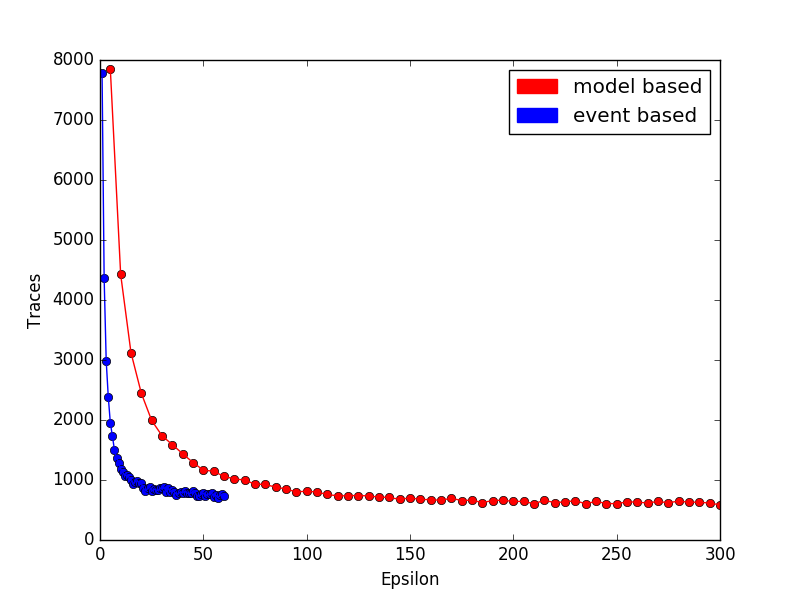
\includegraphics[width=.9\linewidth]{data/BPI2012_lax_vs_strict.png}
	  \caption{BPI2012}
	  \label{fig:eventmodelcomparison12}
	\end{subfigure}%
	\begin{subfigure}{.5\textwidth}
	  \centering
	  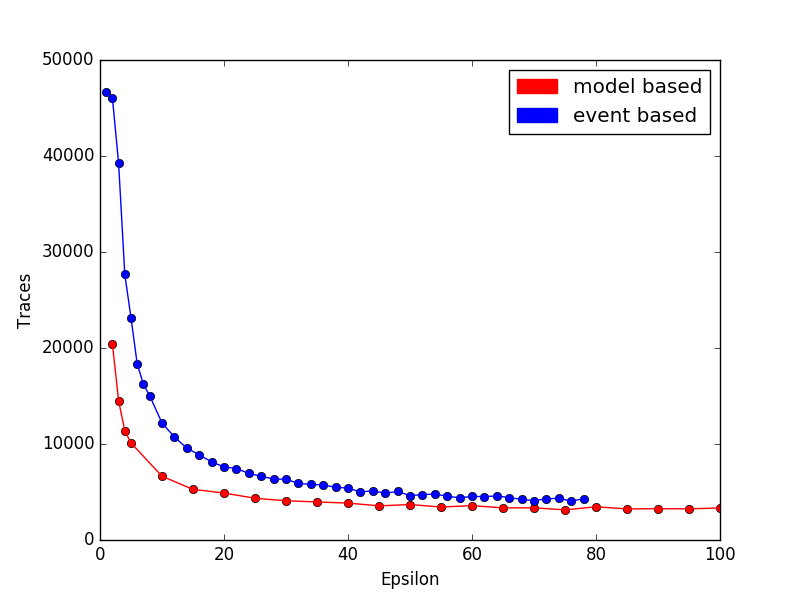
\includegraphics[width=.9\linewidth]{data/BPI2014_lax_vs_strict.png}
	  \caption{BPI2014}
	  \label{fig:eventmodelcomparison14}
	\end{subfigure}
	\caption{Comparison of model based and event based cycle time analysis and it's effect on the total traces with varying $\epsilon$}
	\label{fig:eventmodelcomparison1214}
\end{figure}
Despite the question what cycle time approximation method a user may prefer it is interesting to see whether one method has an advantage over the other on an performance perspective.\\
In \ref{fig:eventmodelcomparison1214} one can see that one can not assume that one method has a smaller or bigger interval of appropriate $\epsilon$, instead one sees that this is also dependent on the distribution of cycle times in te log, which could lead to any of the both methods to have a bigger assortment of viable $\epsilon$.
In \ref{fig:eventmodelcomparison12} one sees that for BPI2012 the cycle times of events do not deviate by a lot. The trace times on the other hand deviate more, which may be a indicator that the number of events in the traces differs a lot and that the log contains many differnt sized traces.\\
In contrast to BPI2014 the analysis of \ref{fig:eventmodelcomparison14} yields that in BPI2012 event times are distributed more randomly, as shown through the impairment on higer $\epsilon$ and that traces have more similar completion times.\\
\begin{figure}[h]
	\begin{subfigure}[t]{.5\textwidth}
	  \centering
	  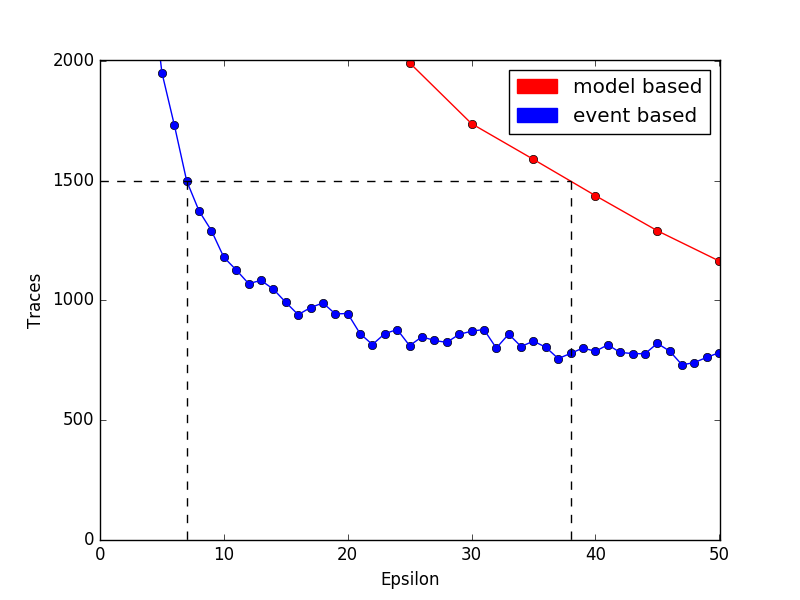
\includegraphics[width=.8\linewidth]{data/lax_vs_strict_traces_epsilon_zoomed.png}
	  \caption{For a model based anylysis $\epsilon$ of 38 and for a event based analysis $\epsilon$ of 7 result in roughly 1500 traces that are seen during pre processing}
	  \label{fig:sametraces12}
	\end{subfigure}%
	\begin{subfigure}[t]{.5\textwidth}
	  \centering
	  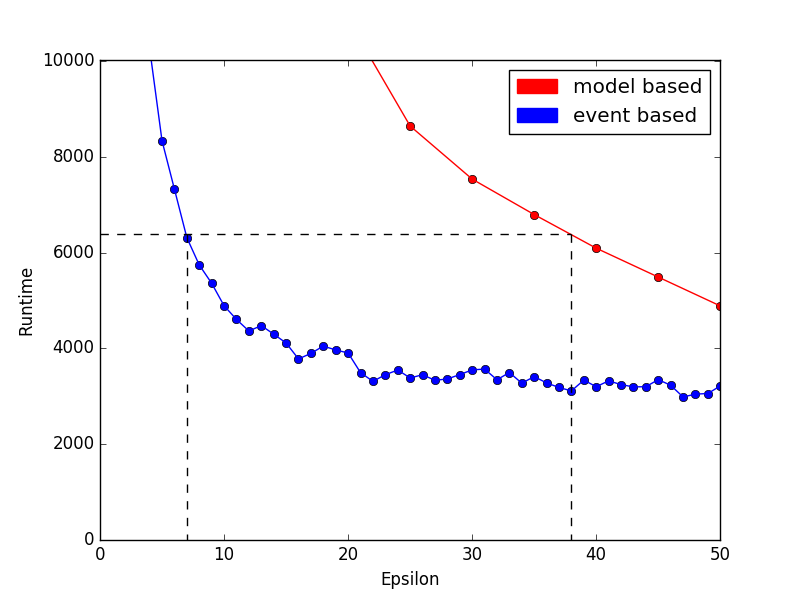
\includegraphics[width=.8\linewidth]{data/kax_vs_strict_runtime_zoomed.png}
	  \caption{For both model based and event based analysis the estimated epsilon result in a 6 second long preprocessing, even though event based analysis has to do more computations}
	  \label{fig:sametime}
	\end{subfigure}
	\caption{Comparing the average runtimes of model based and event based cycle time approximation for $\epsilon$ that result in similar trace numbers for both analysis types for BPI2012.}
	\label{fig:sametimetraces12}
\end{figure}
If one tries to compare the runtime of both analysis techniques then one will see that for $\epsilon$ where both see a similar amount of traces the runtimes are also similar, which contradicts the statement that event based analysis has to do more computations per trace.\\
The algorithm incorporates model based analysis, that has to analyse each event anyway. So no matter wat cycle time approximation is used, in both cases the algorithm has to analyse each event in each seen trace anyway because of the model criteria, so the drawback of event based analysis is actually irrelevant for the algorithm and none of both techniques has a visible computational advantage over the other.\\
As a computational difference is non existent both techniques should be presented to the user, who should then decide which method best fits his needs.
\subsubsection{Fitness}
\begin{figure}[h]
	\begin{subfigure}{.49\textwidth}
	  \centering
	  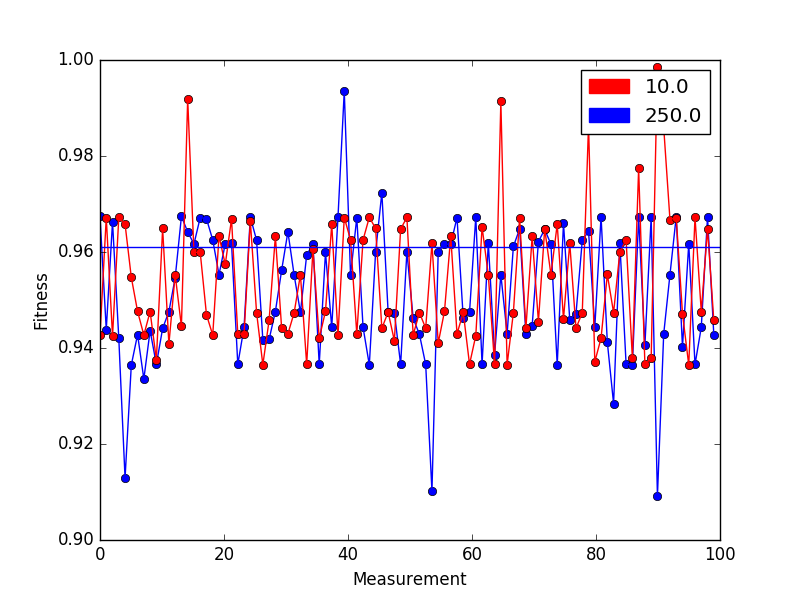
\includegraphics[width=.8\linewidth]{data/BPI2012/lax_10_250_fitness.png}
	  \caption{Fitness comparison for a model based cycle time approximation for $\epsilon$ of 10 and 250, BPI 2012}
	\end{subfigure}%
	\begin{subfigure}{.49\textwidth}
	  \centering
	  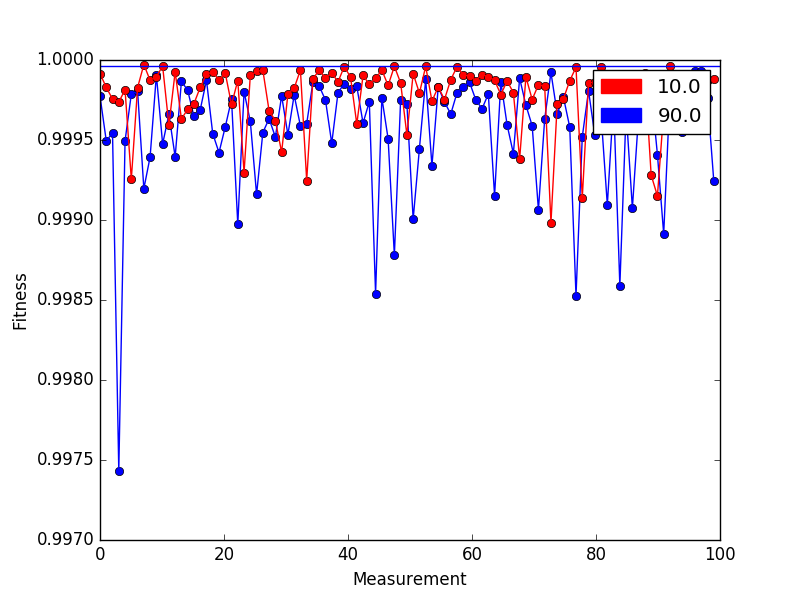
\includegraphics[width=.8\linewidth]{data/BPI2014/lax_10_90_fitness.png}
	  \caption{Fitness comparison for a model based cycle time approximation for $\epsilon$ of 10 and 90, BPI 2014}
	  \label{fig:fitnessStrict12}
	\end{subfigure}
	\caption{Fitness Measurements for BPI2012 and 2014}
	\label{fig:fitness1214}
\end{figure}
sIMi does not loose a lot of fitness compared to IMi which seems to be due to the fact that sIMi is more likely to leave out the traces that are infrequent while all seen infrequent traces will be filtered out anyway, so in average both would yield the same result and a similar fitness score. Due to the random nature of picking traces there are also some cases where sIMi reaches a higher fitness score.\\
Even though the algorithm has similar fitness values as IMi the model differ slightly for multiple runs of the algorithm, which is again due to the random trace picking nature.
In the worst case this could lead to a user being confused, as he would normally assume that the algorithm creates the same model each run. See \ref{fig:processTree12} for an example.
This should be prevented, e.g. by changing the algorithm to pseudo randomly pick traces by using seeds and forcing the algorithm to choose the same traces again for the same log by using the same seed again.
\begin{figure}[h]
\centering
	\begin{subfigure}{.7\textwidth}
	  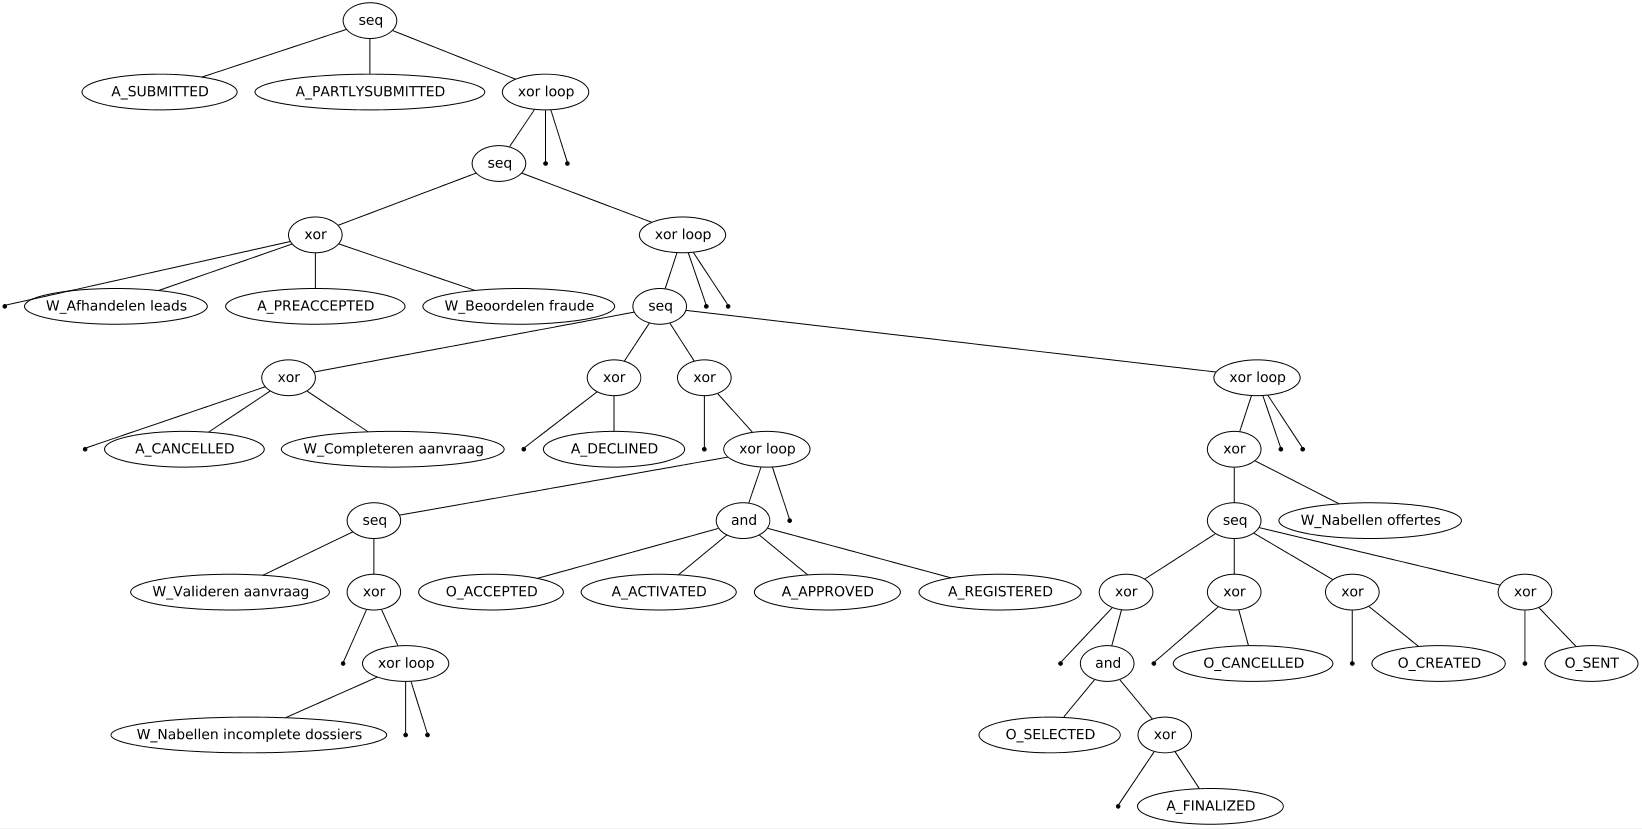
\includegraphics[width=\linewidth]{data/process_tree_2.png}
	\end{subfigure}\vspace{0.5cm}
	\centering
	\begin{subfigure}{.7\textwidth}
	  \centering
	  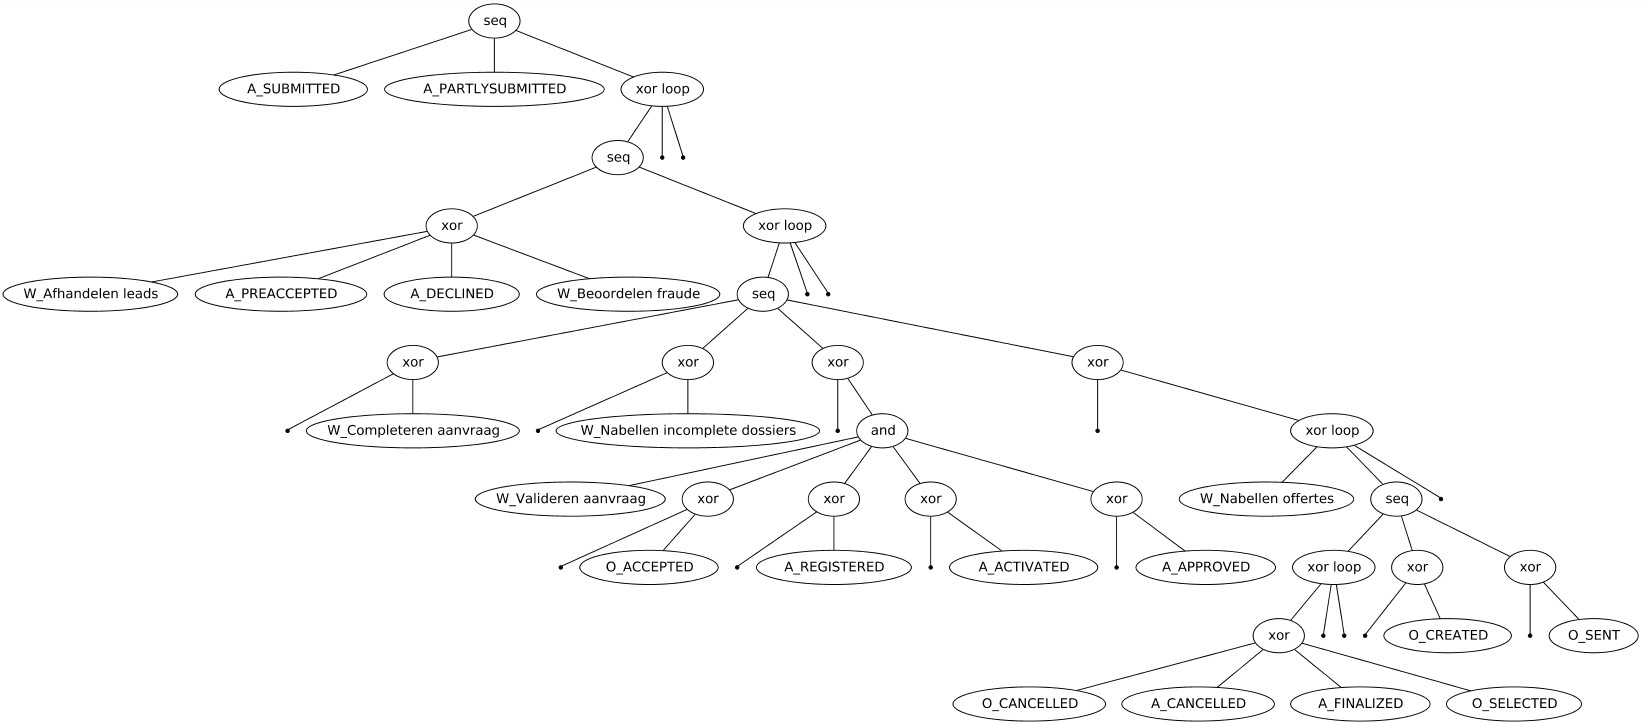
\includegraphics[width=\linewidth]{data/process_tree_3.png}
	\end{subfigure}
	\caption{Two with sIMi mined Process Trees using 0.2 as the filter threshold, BPI2012. One can clearly see that the two trees are structurally different}
	\label{fig:processTree12}
\end{figure}
\subsection{Analyzing a Log's Influence on Performance}
\subsubsection{Using Block Structures to determine Best Case Performance}
So far analysis has been done on how well sIMi competes against IMi, but the logfiles influence on the runtime is still unknown.\\ As mentioned multiple times already, the runtime is dependent on the amount of new information seen in traces, which on a strict model basis is dependent on the number of events, starting-, end-events and edges that would be present in the final directly follows graph. If log a contains double the amount of edges or vertices than log b, one can easily assume that the analysis of log a will take longer, as the end of the preprocessing will be prolonged roughly twice as often as for log b.\\
\begin{wrapfigure}{r}{0.5\textwidth}
  \vspace{-20pt}
	\begin{center}
		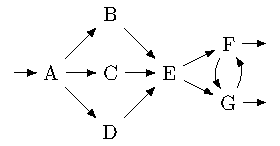
\includegraphics{img/petriNet_traceCoverage.pdf}
	\end{center}
	  \vspace{-10pt}
	\caption{A Directly follows graph of an imaginary log containing 7 vertices, 9 edges, 1 starting node and 2 end nodes. The traces <ABEFG>,<ACEFG>,<ADEGF> contains all these informations and are therefore enough to represent this graph.}
	\label{fig:directlyFollowsCoverageExample}
\end{wrapfigure}
~\cite{InductiveMiner} describes how all process tree operators are represented through certain edge combinations in the directly follows graph. Each of these operators represents a block in the block structured end model. Therefore one can try to analyze how much information is present in a certain type of block and try to conclude what the minimal amount of traces is that can describe the behaviour that is present in the block. Because behavior can be represented through edges that a trace takes through the graph, one just needs to find out the minimal number of traces that incorporate all edges of the block like shown in \ref{fig:directlyFollowsCoverageExample}.
As each block is described through the interactions between it's subblocks a prediction or at least approximation of the minimal amount of traces that IMi has to see can be done.\\
\paragraph{Single Events}
This is the base case as a single event does not contain other block stuctures. A single event takes at least one trace.\\
\paragraph{Sequences}
Sequences are concatenations of possible paths through all subblocks of the sequence block. Each path in a block begins at a start node and ends at an ending node. As some subblocks have the need for more paths than others and as all blocks have to be traversed in a sequence, the block with the highest trace requirement determines how many traces are required in a block as this trace number could incorporate all other blocks minimal trace number. In \ref{fig:directlyFollowsCoverageExample} this has been used implicitly. The graph is a sequence of an event, a 3-event xor-cut, another event and a 2-event and-cut. In this scenario the xor-cut has the highest trace requirement, as 3 traces are needed to see each of B,C and E and the other possible paths through the other blocks can be covered in these 3 different traces.\\
For two blocks, where block A preceeds block B, each ending node of block A has an edge to each starting node of block B. As a path through a block ends with and starts with exactly one node of the appropriate set the algorithm needs at least as many traces as the product of ending nodes of block A times the starting nodes of block B.\\ Therefore either the most requiring subblock or the most requiring node product between sequential blocks depicts the total minimal amount of traces needed for the sequence block. \ref{fig:sequenceTraces} visualizes these two possibilities.\\
\begin{figure}[h]
	\begin{subfigure}[t]{.5\textwidth}
	  \centering
	  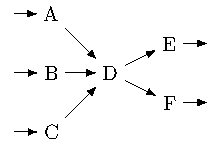
\includegraphics[width=.55\linewidth]{img/sequence_xor_event_xor.pdf}
	  \caption{A sequence of a 3-event-xor, a single event and a 2-event-xor. Here the most requiring factor for the block is the first xor-block, thus requiring at least 3 traces to discover all information(i.e <ADE>,<BDF>,<CDE>)}
	  \label{fig:sequenceXorEventXor}
	\end{subfigure}
	\begin{subfigure}[t]{.5\textwidth}
	  \centering
	  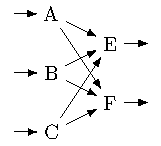
\includegraphics[width=.4\linewidth]{img/sequence_xor_xor.pdf}
	  \caption{Two sequential xor-blocks. Here the 6 edges between the two blocks necessitate at least 6 traces to see all information in the graph (i.e <AE>,<AF>,<BE>,<BF>,<CE>,<CF>)}
	  	  \label{fig:sequenceXorXor}
	\end{subfigure}
	\caption{Two directly follows graphs that are structured as sequences with varying minimal trace requirements}
	\label{fig:sequenceTraces}
\end{figure}
\paragraph{Loops}
Loops are a special case. In theory no matter how interleaving loops are and no matter what subblocks they contain and how many paths they require in order to detect all information, a single trace can take multiple paths through the loop and so all information inside the loop can be detected in one trace. The more interleaved the loop is the more unlikely it becomes that a trace contains all information, but the possibility always persists. As seen exemplary in \ref{fig:loopCoverageExample} 1 can be assumed as the minimal amount of traces.
\begin{figure}[h]
  \vspace{-20pt}
	\begin{center}
		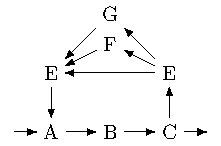
\includegraphics[width=.3\linewidth]{img/loop.pdf}
	\end{center}
	  \vspace{-10pt}
	\caption{A directly follows graph depicting a loop that contains a second loop with a xor-block in it's optional part. Even though 2 traces are needed to see all information for the xor-block in isloation, the trace <ABCDEABCDFABCDGABC> conatins all information seen in the graph.}
	\label{fig:loopCoverageExample}
\end{figure}
\paragraph{Xor-Blocks}
A xor-block has multiple paths and a trace has to take exactly one path. Therefore the minimal trace requirement of a xor-block is the sum of the requirements of all it's subblocks. 
\begin{figure}[h]
  \vspace{-20pt}
	\begin{center}
		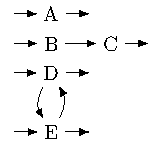
\includegraphics[width=.25\linewidth]{img/xor.pdf}
	\end{center}
	  \vspace{-10pt}
	\caption{A directly foloows graph structured as a xor-block. For the first two paths one trace is needed, for the third path 2 traces are needed, so the traces <A>,<BC>,<DE> and <ED> include all information.}
	\label{fig:xorCoverageExample}
\end{figure}
\paragraph{And-Blocks}
In and-blocks there exists a path between all nodes of different subblocks in the graph.
As the possible edges in such a graph change drastically with the number of events in subblocks and depending on what type of subblocks are present, it is very difficult to give a correct estimation on the minimal number of traces that contain all information. The more events an and-block contains the more informaton is needed to detect it completely (as for $|V|$ vertices in the graph up to $|V|$ edges could be added we addif  a new event is added), so one can assume the minimal required traces to grow factorial with the number of events in the and-block.
\begin{figure}[h]
  \vspace{-20pt}
	\begin{center}
		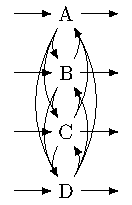
\includegraphics[width=.2\linewidth]{img/and.pdf}
	\end{center}
	  \vspace{-10pt}
	\caption{A directly follows graph containing a simple and-block. The traces <ACDB>,<BADC>,<CABD>,<DCBA>,<BCDA> can represent all information.}
	\label{fig:andExample}
\end{figure}\\\\
Having estimated the minimal number of traces a block needs to see in order to see all information one can conclude that and-structures in a log influence the runtime very badly the bigger they are, while sequences of complex structures and xor-blocks containing other complex stuctures add notably to the runtime.\\
\subsubsection{Noise and Cycle Times Deviation}
\paragraph{Noise}
Even though noise will be filtered out in the end and does not affect the end model, it prolongs the pre processing chain should it be seen in the log. The more noise a log contains the longer the runtime will be, as more traces have to be seen until the pre processing stops. \ref{fig:noise} depicts this assumption.
\begin{figure}[h]
	\begin{center}
		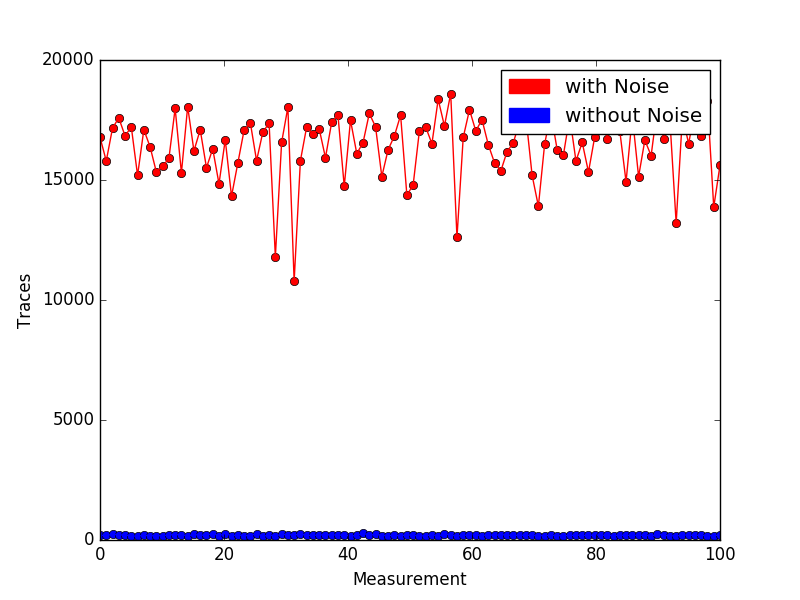
\includegraphics[width=.5\linewidth]{img/Noise_Noiseless.png}
	\end{center}
	  \vspace{-10pt}
	\caption{Comparison of read traces for a randomly generated log once with and once without added noise}
	\label{fig:noise}
\end{figure}
\paragraph{Cycle Time Deviation}
Smaller $\epsilon$ increase the runtime of the algorithm. Logs for which the completion time of events or traces deviate by a lot will result in a longer runtime than those where the average deviation is smaller. This is depicted in \ref{fig:deviation}, as the cycle time approximation takes longer in tese cases.
\begin{figure}[h]
	\begin{center}
		\includegraphics[width=.5\linewidth]{img/high_vs_low_deviation.png}
	\end{center}
	  \vspace{-10pt}
	\caption{Comparison of read traces for a randomly generated log with differing deviations of cycle times. Measurements have been taken with $\epsilon$ of 30s and all deviations were uniformly distributed between the time limits.}
	\label{fig:deviation}
\end{figure}
\section{Conclusion}
In this work I presented an alghorithmic framework that added a preprocessing step to the Inductive Miner infrequent algorithm that uses statistical log analysis in order to reduce the number of traces that IMi has to use, effectively reducing the input size. The preprocessing considered model correctness and an approximative cycle time correctness as the defining factors to conclude the size of the new sublog.
I showed that the so created statistical Inductive Miner infrequent - sIMi, is faster and more memory efficient for a large amount of input data, while achieving similar fitness values as IMi. Only for very strict cycle time approximation does the algorithm take longer than IMi, therefore the algorithm has an advantage against IMi in real life scenarios and is more scalable than aforementioned algorithm if the user is able to specify a good threshold for the cycle time approximation. The only redeeming factor is that sIMi produces differing models for same inputs even if the qualitative dimensions do not suffer.\\
Furthermore I showed that a too strict cycle time approximation is not beneficial to the algorithms runtime. Logs that contain big and-structures have the higest runtimes, followed by sequences of complex workflow constructs and xor-blocks containing complex event structures. Noise or high cycle time deviations also increase the runtime.\\\\

As an outlook, further work should be done on guaranteeing that the same model is discovered for same inputs. To achieve this the random number generator would have to be initialized in such a way that it uses the same seed for the same log. Further work has to be done on improving the runtime upon strict cycle time approximation.
\section{Appendix}
\subsection{Using statistical Inductive Miner infrequent}
The code of sIMi can be found at\\
\url{https://github.com/Martin-Bauer/StatisticalInductiveMinerInfrequent}.\\\\
For further instructions see the readme-file in the link.
\newpage


\bibliography{BA_bib.bib}{}
\bibliographystyle{ieeetr}
% Erzeugen der Selbständigkeitserklärung auf einem neuen Blatt:
\selbstaendigkeitserklaerung{\today}
\end{document}
